\documentclass[a4paper]{article}

%% Language and font encodings
\usepackage[english]{babel}
\usepackage[utf8x]{inputenc}
\usepackage[T1]{fontenc}
\usepackage{outlines}
\usepackage{amsfonts}
\usepackage{dsfont}
\usepackage[ruled,vlined]{algorithm2e}

%% Sets page size and margins
\usepackage[a4paper,top=3cm,bottom=2cm,left=3cm,right=3cm,marginparwidth=1.75cm]{geometry}

%% Useful packages
\usepackage{amsmath}
\usepackage{graphicx}
\usepackage[colorinlistoftodos]{todonotes}
\usepackage[colorlinks=true, allcolors=blue]{hyperref}

\usepackage{amsthm}
\theoremstyle{plain}

\newtheorem*{remark*}{Remarque}
\newtheorem*{conclusion*}{Conclusion}
\newtheorem*{theorem*}{Théorème}
\newtheorem{theorem}{Théorème}

%% For paragraphs to be correctly indented
\setcounter{secnumdepth}{5}
\newcommand{\myparagraph}[1]{\paragraph{#1}\mbox{}\\}

%% For Underbars
\usepackage{accents}
\newcommand{\ubar}[1]{\underaccent{\bar}{#1}}

%% Double brackets
\usepackage{stmaryrd}

\title{Machine Learning supervisé}
\author{Léonard Binet}

\begin{document}
\maketitle

\begin{abstract}
Synthèse, reformulation et interprétation des différents cours de Machine Learning, avec une harmonisation des notations et conventions. La partie "sélection de modèle" s'affranchit plus librement des cours et est à considérer peut-être avec un regard plus critique.
\end{abstract}


\pagebreak
\tableofcontents




\pagebreak
\section{Cadre de la classification supervisée}

\subsection{Introduction}

L'objectif de la classification est de pouvoir prédir l'étiquette d'une observation à partir de ses variables explicatives, après s'être entraîné sur un ensemble d'entraînement.\\
Le résultat d'une démarche de classification est l'obtention d'un "classifieur", qui est une fonction qui prend en entrée les variables explicatives d'une observation, et renvoie une prédiction d'étiquette.\\

\subsubsection{Enjeux}

Nous disposons d'un ensemble d'apprentissage constitué d'observations labelisées, c'est à dire d'observations disposant simultanément de variables explicatives, et d'étiquettes.

L'objectif de notre démarche est de prédire au mieux l'étiquette des futures observations non labelisées. Pour cela nous allons essayer de trouver à partir de notre ensemble d'apprentissage un \textbf{classifieur}, qui à partir de variables explicatives d'une observation nous propose une étiquette.

Logiquement, nous chercherons à minimiser les erreurs de prédiction commises par notre classifieur.

Cependant, même dans l'hypothèse où nous arriverions à prédire parfaitement sur notre jeu de données, cela ne signifierait pas pour autant que la démarche a abouti avec succès. 

En effet, suivant la liberté que nous nous donnons dans le choix du classifieur, il est possible si nous acceptons une complexité sans borne dans notre classe de classifieurs, de trouver un classifieur qui "colle" parfaitement à notre ensemble d'entraînement, mais qui ne se généralise pas à d'autres données.

Un enjeu majeur est donc comprendre les fondements de la capacité de généralisation de notre classifieur à des données qu'il n'a pas observées.

Le sujet du nombre d'operations, et du temps computationel pour faire converger l'algorithme ne sera pas évoqué.

\subsubsection{Etapes}


\begin{outline}
\1 Définition du cadre probabiliste et interpretation du conditionnement de X et Y.
\1 Formalisation de la recherche de notre classifieur et des notions de coût et de risque.
\1 Existence d'un classifieur optimal.
\1 Introduction des données et de la démarche d'estimation du classifieur optimal (dont algorithmie).
\1 Conditions de la pertinence de l'utilisation du classifieur obtenu par minimisation du risque empirique, sur d'autres données issues de la même loi de probabilité.
\1 Recherche et évaluation du classifieur optimal (minimisant le risque 'réel' de généralisation).
\1 Détail des différents types de classifieurs.
\end{outline}

\subsubsection{Vue d'ensemble des notations:}

C'est une première présentation des notations, elles seront toutes redifinies progressivement.

\begin{outline}

\1 Cadre probabiliste:
\2 X un vecteur aléatoire à valeurs dans $\mathcal{X} \subset \mathbb{R}^p$
\2 Y une variable aléatoire dicrète à valeurs dans $\mathcal{Y} $, avec $|\mathcal{Y}|$ fini.


\2 P la loi de probabilite jointe des variables aléatoires $(X,Y)$ (inconnue).



\1 Notations de classification : probabilité, côté "théorique"

\2 $f: \mathcal{X} \rightarrow \mathcal{Y}$ par ex. $ \mathbb{R}^p \rightarrow \{-1,1\} $ une fonction appelée classifieur, qui pour un point $x \in \mathcal{X}$ fournit une étiquette  $f(x) \in \mathcal{Y}$.

\2 $\mathcal{F}$, une classe de fonctions, parmi lesquelles nous allons chercher notre classifieur.

\2 $ \mathit{l}: x, f(x), y \in (\mathcal{X}, \mathcal{Y}, \mathcal{Y}) \rightarrow \mathbb{R} $ une fonction de perte qui mesure le coût d’une erreur lors de la prédiction d’un exemple (à partir, des features, du label, et de la prédiction). La version la plus simple: $l(X,Y,f(X))= \mathds{1}_{Y\neq f(X)}$ (1 si le classifieur se trompe, 0 s'il a raison).

\2 $R(f)= \mathbb{E}_P(l(X,Y,f(X)))$ le risque du classifieur $f$ sur $P$. Dans la version la plus simple, si $l(X,Y,f(X))= \mathds{1}_{Y\neq f(X)}$, alors $R(f)= \mathbb{P}(f(X)\neq Y)$. Ce risque est conditionné à la probabilité P et à la fonction de coût $l$ (ce risque est aussi appelé risque de généralisation).
 
 \2 $\bar f \in {\rm arg} \displaystyle\min_{f \in \mathcal{F}} R(f) $, c'est à dire un classifieur qui minimise le 'vrai' risque sur notre classe de fonction $\mathcal{F}$ (ie: $R(\bar f) = R_{\mathcal{F}}$).

\2 $f^{\ast} \in {\rm arg} \displaystyle\min_{f} R(f) $ un classifieur qui minimise le vrai risque, sans contrainte de classe pour notre classifieur.

\1 Notations de classification : estimation, "côté empirique"

\2 $ \mathcal{D}_n = \{(x_i, y_i), i \in 1,n\} \in (\mathcal{X},\mathcal{Y})^n$ un ensemble d’apprentissage contenant $n$ observations et leurs étiquettes, que nous supposons $iid$ et issues de P, la loi de probabilité de (X,Y). On notera $P_{\mathcal{D}_n}$ la loi de probabilité de l'échantillon dans son ensemble.


\2 $\hat R(f, \mathcal{D}_n)$, le risque empirique, un estimateur du risque 'réel' de $f$, $R(f)$, estimé à partir de l'échantillon $\mathcal{D}_n$ (erreur sur l'ensemble d'apprentissage). En général: $$\hat R_n(f, \mathcal{D}_n) = \frac{1}{n}\sum_{i=1}^{n}\mathit{l}(x_i,y_i,f(x_i))$$

\2 $\mathcal{A}$ l'algorithme (procédure d'estimation) nous permettant à partir de notre ensemble d'entraînement $\mathcal{D}_n$ de trouver un classifieur $\hat f$, qui soit un estimateur du classifieur minimisant le risque empirique. Ie: $\hat f = \mathcal{A}(\mathcal{D}_n) $. Pour être exhausif, en réalité $\mathcal{A}$ dépend également de la classe considérée, et de la fonction de coût choisie. Ainsi on pourrait noter: $\hat f = \mathcal{A}(\mathcal{D}_n,\mathcal{F},l)$. En s'avançant sur les notations plus précises à venir sur les risques, $\hat f$ est un estimateur de $\bar f$, le classifieur  minimisant le risque 'réel' sur $\mathcal{F}$.

\2 $\hat f_n \in \mathcal{F}$ le classifieur trouvé en minimisant le risque empirique $\hat R_n$ sur l'ensemble d'apprentissage $\mathcal{D}_n$ avec l'algorithme $\mathcal{A}$. C'est notre estimateur de $\bar f$.


\end{outline}

\subsection{Définition du cadre probabiliste}
Nous supposons qu'il existe une fonction $f$ telle que: 
$$ y = f(X) + \epsilon$$

\begin{outline}

\1 Cadre probabiliste:
\2 X un vecteur aléatoire à valeurs dans $\mathcal{X} \subset \mathbb{R}^p$
\2 y une variable aléatoire dicrète à valeurs dans $\mathcal{Y} $, avec $|\mathcal{Y}|$ fini.
\2 P la loi de probabilite jointe des variables aléatoires $(X,y)$, (inconnue).
\2 $\epsilon$ une variable aléatoire correspondant à un bruit

\end{outline}

Supposons que nous cherchions à déterminer le type de fleur à partir de plusieurs de ses caractériques (variables explicatives numériques), par exemple la taille de ses pétales, et la longueur de sa tige.

Le vecteur aléatoire X caractérise les p variables explicatives d'un individu(ici taille de pétale, longueur de tige). La variable Y représente son étiquette (ie le type de fleur). Nous cherchons à déterminer l'étiquette, à partir de la connaissance des variables explicatives. 

Alors, notre démarche consiste à déterminer Y, (inconnu, type de fleur), sachant X = $x_{connu}$ (sachant les caractistiques de la fleur).

Notons ici que cette démarche n'a d'intérêt que s'il existe réellement un lien entre X et Y. S'il s'avère que X et Y sont indépendantes, alors la connaissance de X ne nous apportera aucune connaissance sur Y.

\subsection{Formalisation de la recherche de notre classifieur}

Plus précisément, nous souhaitons définir une fonction, qui à chaque individu, puisse associer une étiquette $y$ qui soit la plus probable sachant $X=x$.

Pour savoir si nous sommes dans la bonne voie, nous souhaitons pouvoir noter la pertinence de notre fonction, par une fonction qui mesure sa réussite sur un individu, et par extension dégager une notion de risque du classifieur.


\begin{outline}
\1 Définissons les notations suivantes:

\2 $f: \mathcal{X} \rightarrow \mathcal{Y}$ par ex. $ \mathbb{R}^p \rightarrow \{-1,1\} $ une fonction appelée classifieur, qui pour un point $x \in \mathcal{X}$ fournit une étiquette  $f(x) \in \mathcal{Y}$.

\2 $ \mathit{l}: x, f(x), y \in (\mathcal{X}, \mathcal{Y}, \mathcal{Y}) \rightarrow \mathbb{R} $ une fonction de perte qui mesure le coût d’une erreur lors de la prédiction d’un exemple (à partir, des features, du label, et de la prédiction). La version la plus simple: $l(X,Y,f(X))= \mathds{1}_{Y\neq f(X)}$ (1 si le classifieur se trompe, 0 s'il a raison).

\2 $R(f)= \mathbb{E}_P(l(X,Y,f(X)))$ le risque du classifieur $f$ sur $P$. Dans la version la plus simple, si $l(X,Y,f(X))= \mathds{1}_{Y\neq f(X)}$, alors $R(f)= \mathbb{P}(f(X)\neq Y)$. Ce risque est conditionné à la probabilité P et à la fonction de coût $l$.
 
\end{outline}

\textbf{Notre objectif est donc, de trouver un classifieur qui minimise le risque $R$.}

\subsection{Existence d'un classifieur optimal: classifieur de Bayes}

\textbf{Problématique: }


Etant donnee $P$ la loi de probabilite jointe de (X,Y), existe-t-il un classfieur $f$ minimisant le risque $R(f)$? (ie tel que):
$$f^{\ast} = {\rm arg} \displaystyle\min_{f} R(f)  $$

La réponse est oui: le classifieur de Bayes:
$$f_{Bayes}(x) = {\rm arg} \displaystyle\max_{y \in \mathcal{Y}} P(Y=y|x)$$

Sa définition est intuitive, en effet, pour un $x_{connu}$ fixé, nous souhaitons connaître le $y$ qui maximise la probabilité $P(Y=y|X=x_{connu})$ que le label soit $y$ \textbf{sachant} $x_{connu}$.

On ne peut pas obtenir un risque plus petit que le risque
bayesien: $R(f_{Bayes})$ qui est une caracteristique du problème.\\

\textbf{Remarque:} dans le cas où X et Y seraient indépendantes, alors: 
$$f^{\ast}(x) = f_{Bayes}(x) = {\rm arg} \displaystyle\max_{y \in \mathcal{Y}} \left(P(Y=y)\times P(X=x) \right) = {\rm arg} \displaystyle\max_{y \in \mathcal{Y}} P(Y=y) $$ 
(par indépendance, puis car $P(X=x)$ constante) On voit que notre meilleur classifieur ne dépend pas de X.\\

\textbf{Nouvelle notation:}

\begin{outline}

\1 $f^{\ast} = {\rm arg} \displaystyle\min_{f} R(f) $ le classifieur de Bayes qui minimise le vrai risque.
\1 $\eta (x) = P(Y|X=x)$, ainsi, $ \forall x \in \mathcal{X}, \quad \eta(x) \in ]0,1[$, est la distribution à posteriori de $Y$ par rapport à $X$.

\end{outline}

\textbf{Problème:} le problème est que ne connaissant pas P, on ne peut pas calculer le risque $R$ ni obtenir directement $f^{\ast}$. Cela reste tout de même notre objectif de se rapprocher de $f^{\ast}$. Et nous allons chercher à l'estimer.

\subsection{Introduction des données et estimation du classifieur optimal}
Supposons que l'on dispose d'un ensemble d'apprentissage $\mathcal{D}_n$ d'observations labelélisées issues de P.  

Nous allons chercher à définir un estimateur qui puisse se rapprocher du classifieur optimal. 

Cependant, ne pouvant pas minimiser le risque 'réel' nous allons à défaut avoir besoin pour cela de définir un estimateur $\hat R_n$ du risque réel $R$ que nous voulons minimiser (une version empirique du risque). Puis il faudra définir une procédure d'estimation $\mathcal{A}$ (algorithme) pour obtenir un estimateur $\hat f_n$ du classifieur optimal, par la minimisation du risque empirique. Dans les faits, on ne connait d'algorithmes que pour estimer des classifieurs dans des classes de fonctions données, que l'on notera $\mathcal{F}$.
\\

\textbf{Nouvelles notations:}

\begin{outline}

\1 $ \mathcal{D}_n = \{(x_i, y_i), i \in 1,n\} \in (\mathcal{X},\mathcal{Y})^n$ un ensemble d’apprentissage contenant $n$ observations et leurs étiquettes, que nous supposons $iid$ et issues de P, la loi de probabilité de (X,Y).

\1 $\mathcal{F}$, une classe de fonctions, parmi lesquelles nous allons chercher notre classifieur.

\1 $\hat R(f, \mathcal{D}_n)$, le risque empirique, un estimateur du risque 'réel' de $f$, $R(f)$, estimé à partir de l'échantillon $\mathcal{D}_n$. En général: $$\hat R_n(f, \mathcal{D}_n) = \frac{1}{n}\sum_{i=1}^{n}\mathit{l}(x_i,y_i,f(x_i))$$

\1 $\mathcal{A}$ l'algorithme (procédure d'estimation) nous permettant à partir de notre ensemble d'entraînement $\mathcal{D}_n$ de trouver un classifieur $\hat f$, qui soit un estimateur du classifieur minimisant le risque empirique. Ie: $\hat f = \mathcal{A}(\mathcal{D}_n) $. Pour être exhausif, en réalité $\mathcal{A}$ dépend également de la classe considérée, et de la fonction de coût choisie. Ainsi on pourrait noter: $\hat f = \mathcal{A}(\mathcal{D}_n,\mathcal{F},l)$. En s'avançant sur les notations plus précises à venir sur les risques, $\hat f$ est un estimateur de $\bar f$, le classifieur  minimisant le risque 'réel' sur $\mathcal{F}$.

\1 $\hat f_n \in \mathcal{F}$ le classifieur trouvé en minimisant le risque empirique $\hat R_n$ sur l'ensemble d'apprentissage $\mathcal{D}_n$ avec l'algorithme $\mathcal{A}$. C'est notre estimateur de $\bar f$.

\1 $\bar f \in {\rm arg} \displaystyle\min_{f \in \mathcal{F}} R(f) $, c'est à dire un classifieur qui minimise le 'vrai' risque sur notre classe de fonction $\mathcal{F}$ (ie: $R(\bar f) = R_{\mathcal{F}}$).

\end{outline}

\textbf{Bilan:}

A défaut de pouvoir minimiser le risque $R$ nous définissons une procédure d'estimation $\mathcal{A}$ pour trouver le classifieur qui minimise $\hat R_n$. Cela soulève deux interrogations principales: 
\begin{outline}

\1 Est ce que l'algorithme $\mathcal{A}$ est \textbf{consistant}, c'est à dire, est ce que le risque réel  $R(\hat f_n)$ du classifieur obtenu par estimation converge effectivement vers le risque réel $R(\bar f)$ du classifieur optimal sur $\mathcal{F}$? Grossièrement, est ce que l'algorithme fait bien son travail d'estimation.
\2 Tout algorithme de minimisation du risque empirique est consistant, ce point n'est donc pas spécifiquement bloquant en général.
\1 Par ailleurs, même dans le cas où l'algorithme est consistant, est ce que le risque 'réel' $R(\hat f_n)$ est maîtrisé? En effet nous nous sommes souciés de minimiser le risque empirique $\hat R_n$, mais rien ne prouve pour l'instant que minimiser ce risque empirique va maîtriser notre risque 'réel'.
\2 C'est la problématique majeure du \textbf{surapprentissage}: le classifieur est très performant sur l'ensemble d'apprentissage, mais ne parvient pas à se généraliser à de nouvelles données.

\end{outline}

\textbf{Nouvel objectif:}

Nous souhaitons trouver dans quel mesure on peut maîtriser le risque 'réel' $R(\hat f_n)$ du classifieur obtenu par notre procédure d'estimation $\mathcal{A}$. Intuitivement, on sent que plus on accepte des classifieurs 'complexes', plus ceux-ci pourront 'coller' aux données d'apprentissage, mais ne pourront pas se généraliser.

\subsection{Conditions de la pertinence de l'utilisation du classifieur obtenu par minimisation du risque empirique, sur d'autres données issues de la même loi de probabilité}


On cherche donc à maîtriser le risque 'réel' de notre classifieur, $R(\hat f_n)$. 
$$R(\hat f_n) = \mathbb{E}_P(l(X,Y,\hat f_n(X)))$$
Si $l(X,Y,f(X))= \mathds{1}_{Y\neq f(X)}$, alors $R(\hat f_n)= \mathbb{P}(\hat f_n(X)\neq Y)$
\\
Le risque 'réel' de $\hat f_n$ signifie: ayant trouvé un classifieur $\hat f_n$ obtenu à partir des données $\mathcal{D}_n$, voici l'espérance de son erreur (de $\hat f_n$) sur P (loi de probabilité de (X,Y)), c'est à dire 'en général' (pas uniquement sur $\mathcal{D}_n$).\\ 
\\

Il faut bien comprendre que $R(\hat f_n) = \mathbb{E}_P(l(X,Y,\hat f_n(X)))$, est \textbf{une variable aléatoire}. En effet $\hat f_n$ dépend de $\mathcal{D}_n$. On peut donc chercher l'espérance de $R(\hat f_n)$ sur la loi de probabilité de $\mathcal{D}_n$. 

Pour plus de précision on pourrait noter le risque réel (à posteriori du tirage de l'échantillon):
$$R(\hat f_n) = \mathbb{E}_P(l(X,Y,\hat f_n(X))|\mathcal{D}_n)$$


Et noter son espérance (à priori du tirage): $$\mathbb{E}_{\mathcal{D}_n}[R(\hat f_n)] =\mathbb{E}_{\mathcal{D}_n}[ \mathbb{E}_P(l(X,Y,\hat f_n(X))|\mathcal{D}_n)]$$
Cette espérance est quant à elle bien déterministe (sous réserve qu'elle existe et que celle-ci ne tende pas vers l'infini).

C'est ce terme que nous allons tenter de borner pour prouver la pertinence de généraliser notre classifieur à des données auxquelles il n'a pas été confronté.

\subsubsection{Décomposition de l'excès de risque 'réel' de notre classifieur}

\textbf{Décomposition simple}

Nous pouvons décomposer l'excès de risque (différence entre le risque réel du classifieur obtenu sur nos données, et le risque minimal de Bayes) comme ceci: 
$$R(\hat f_n) - R^{\ast} = [R(\hat f_n) - R_{\mathcal{F}}] + [R_{\mathcal{F}} - R^{\ast}]$$

\label{Detail_exces_risque}

\begin{outline}

\1 avec $ R(\hat f_n) - R_{\mathcal{F}} $ l'erreur d'estimation, qui mesure à quel point on s'approche de l'optimum dans $\mathcal{F}$ ("variance" dépendante des données)

\1 et $ R_{\mathcal{F}} - R^{\ast}$ l'erreur d'approximation, inherente a la classe de fonctions choisie et indépendante de notre ensemble d'apprentissage. Par exemple, si la frontiere de séparation est
non lineaire et que je me restreins a un classifieur lineaire (le "biais"). 

\end{outline}

\textbf{Décomposition plus précise}

Nous pouvons décomposer l'excès de risque plus finement comme suit:
$$R(\hat f_n) - R^{\ast} = [R(\hat f_n) - \hat R_n(\hat f_n)] + [\hat R_n(\hat f_n) - \hat R_n(\bar f)] + [\hat R_n(\bar f) -R(\bar f)] + [R(\bar f) - R^{\ast}]$$

Avec:

\begin{outline}

\1 $\hat R_n(\hat f_n) - \hat R_n(\bar f) < 0 $ car par définition $\hat f_n$ minimise le risque empirique.

\1 $R(\hat f_n) - \hat R_n(\hat f_n) < \displaystyle\sup_{f \in \mathcal{F}} |R(f) - \hat R_n(f)| $
\1 $\hat R_n(\bar f) -R(\bar f) < \displaystyle\sup_{f \in \mathcal{F}} |R(f) - \hat R_n(f)|$

\end{outline}

D'où au final:
$$R(\hat f_n) - R^{\ast} \leq 2 \displaystyle\sup_{f \in \mathcal{F}} |R(f) - \hat R_n(f)| + [R(\bar f) - R^{\ast}]$$


On voit que, pour une classe $\mathcal{F}$ donnée:
\begin{outline}
\1 $[R(\bar f) - R^{\ast}] = [R_{\mathcal{F}} - R^{\ast}]$ est fixé et fini, c'est notre "biais", il est indépendant des données
\1 $2 \displaystyle\sup_{f \in \mathcal{F}} |R(f) - \hat R_n(f)|$, qui dépend à la fois de $\mathcal{F}$ et de $\mathcal{D}_n$, est un élément que nous allons chercher à borner. C'est une variable aléatoire (car c'est une fonction de $\mathcal{D}_n$). Si on arrive à borner ce terme, on prouve qu'il est pertinent de généraliser notre classifieur à des données autres que $\mathcal{D}_n$ (Note: il s'avère que ce terme diminue lorsque $n$ augmente, et augmente lorsque la "complexité" de la classe $\mathcal{F}$ augmente. On peut le considérer comme la partie "variance" du risque aux données $\mathcal{D}_n$ tirées) 
\end{outline}

C'est à partir de ce résultat que Vapnik et Chervonenski arrivent à borner l'excès de risque en fonction de la "complexité" de la classe de fonction $\mathcal{F}$.\\

\textbf{Notations:}
\begin{outline}

\1 $R(\hat f_n) - R^{\ast}$ correspond à l'excès de risque du classifieur $\hat f_n$ que nous avons trouvé via un algorithme de minimisation du risque empirique, ie le risque qui dépasse le risque minimum (celui de Bayes).

\end{outline}

\subsubsection{Le risque 'réel', dépendant de la "complexité" d'une classe de fonctions}

\begin{remark*} On trouvera l'ensemble des démonstrations dans "Pattern classification and learning theory" de Gabor Lugosi.
 \end{remark*}

Dans le cas 'très fini' où l'on dispose d'une classe de fonction $\mathcal{F}$ avec un cardinal fini noté $|\mathcal{F}|=N$, on va chercher à borner l'espérance de notre excès de risque par une fonction de $N$. On arrive à borner la partie "variance" par:\\

$$\mathbb{E}[\sup_{f \in \mathcal{F}} |\hat R_n(f) - R(f)|] \leq \sqrt{\frac{log(2N)}{2n}}$$

Dans le cas 'fini' d'une classe de fonction $\mathcal{F}$ avec une dimension finie, (mais un cardinal infini), on va chercher à borner l'espérance de notre excès de risque par une fonction de la dimension de Vapnik Chervonenski, si la dimension de Vapnik Chervonenski de cette classe est finie.\\

En notant: $ V_{\mathcal{F}} = dim_{VC}(\mathcal{F})$ la dimension de Vapnik Chervonenkis de la classe de fonctions $\mathcal{F}$:
$$\mathbb{E}[\sup_{f \in \mathcal{F}} |\hat R_n(f) - R(f)|] \leq 4 \sqrt{\frac{V_{\mathcal{F}} \times log(n+1)+log(2)}{n}}$$

Dans le cas 'infini' où la dimension de notre classe de fonction est infinie, alors on n'arrivera pas à borner l'espérance de l'excès de risque. On arrivera toujours à obtenir un $\hat f_n$ tel que le risque empirique de ce classifieur soit nul, ie $\hat R_n(\hat f_n) = 0$, en revanche le 'vrai' risque $R(\hat f_n)$ ne pourra pas être borné, et on n'arrivera pas à généraliser la prédiction sur des données extérieures à $\mathcal{D}_n$.
\\
$$lim_{n \to \infty} \left(\mathbb{E}[\sup_{f \in \mathcal{F}} |\hat R_n(f) - R(f)|] \right) = + \infty $$

\textbf{Conclusion} 

On a réussi à prouver qu'en minimisant le risque empirique $\hat R_n(f)$ pour $f \in \mathcal{F}$, avec $\mathcal{F}$ de dimensions de Vapnik Chervonenkis finie, on obtient un classifieur $\hat f_n$, dont l'espérance du risque 'réel' est bornée. C'est à dire, il est pertinent de généraliser l'utilisation de ce classifieur sur des données extérieures à notre ensemble d'apprentissage $\mathcal{D}_n$, sous réserves que ces données soient issues de la même loi de probabilité.\\

\textbf{Quelles sont les méthodes à classe $\mathcal{F}$ à dimension finie pour lesquelles cette démonstration s'applique:}
\begin{outline}
\1 Fonctionne pour:
\2 les approches paramétriques de manière générale (SVM, régression logistique, perceptron)
\2 arbres de décision binaire "with perpendicular/diagonal splits"
\2 les techniques générales de partitionnement avec hypercubes 
\2 les séparateurs linéaires (perceptron)
\1 Ne fonctionne pas pour:
\2 SVM non-linéaire
\2 boosting
\2 approches discriminantes (k-plus proches voisins)
\2 méthodes ensemblistes (random-forest, votes à la majorité)
\end{outline}


\textbf{Ce que l'on n'a pas prouvé} 

Cela ne signifie pas pour autant que le classifieur obtenu par minimisation du risque empirique soit celui qui minimise le risque 'réel', ou qu'il soit le meilleur que l'on puisse obtenir. Pour obtenir un classifieur de meilleure qualité sur les données issues de $P$, on va chercher des méthodes plus fines (par exemple en pénalisant la 'complexité' de notre classifieur, ou par des méthodes de validation empiriques).

Si l'on reprend la décomposition 'simple' de l'excès de risque de notre classifieur $\hat f_n$ (cf. \ref{Detail_exces_risque}), celle ci est composée de la somme de deux termes. Un excès de risque inhérent à la classe de fonction $\mathcal{F}$ ("biais"), un autre lié à l'erreur d'estimation de $\bar f$, "variance" dépendante de $\mathcal{D}_n$. C'est ce dernier terme de variance qui va 'exploser' lorsque l'on acceptera des une classe $\mathcal{F}$ trop complexe.\\


\subsubsection{Compromis 'biais'/'variance' pour limiter le surapprentissage}
Il nous faut limiter le biais, mais éviter le surapprentissage ("variance" à l'ensemble d'apprentissage $\mathcal{D}_n$).

\begin{outline}

\1 Si la classe $\mathcal{F}$ est trop petite, on ne peut pas atteindre la cible (biais large)

\1 Si la classe $\mathcal{F}$ est trop grande, on ne peut pas reduire la variance de l'estimateur (variance trop importante)
\end{outline}

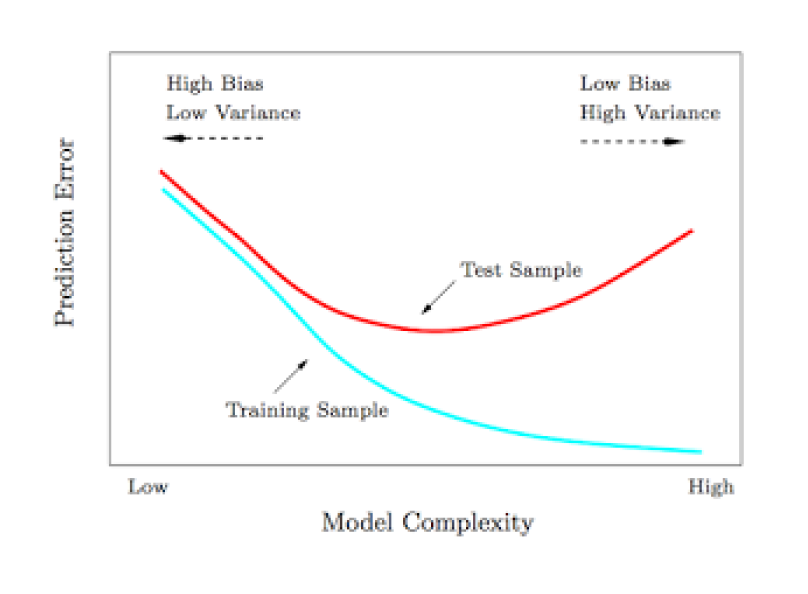
\includegraphics[width=13cm]{Overfitting.png}

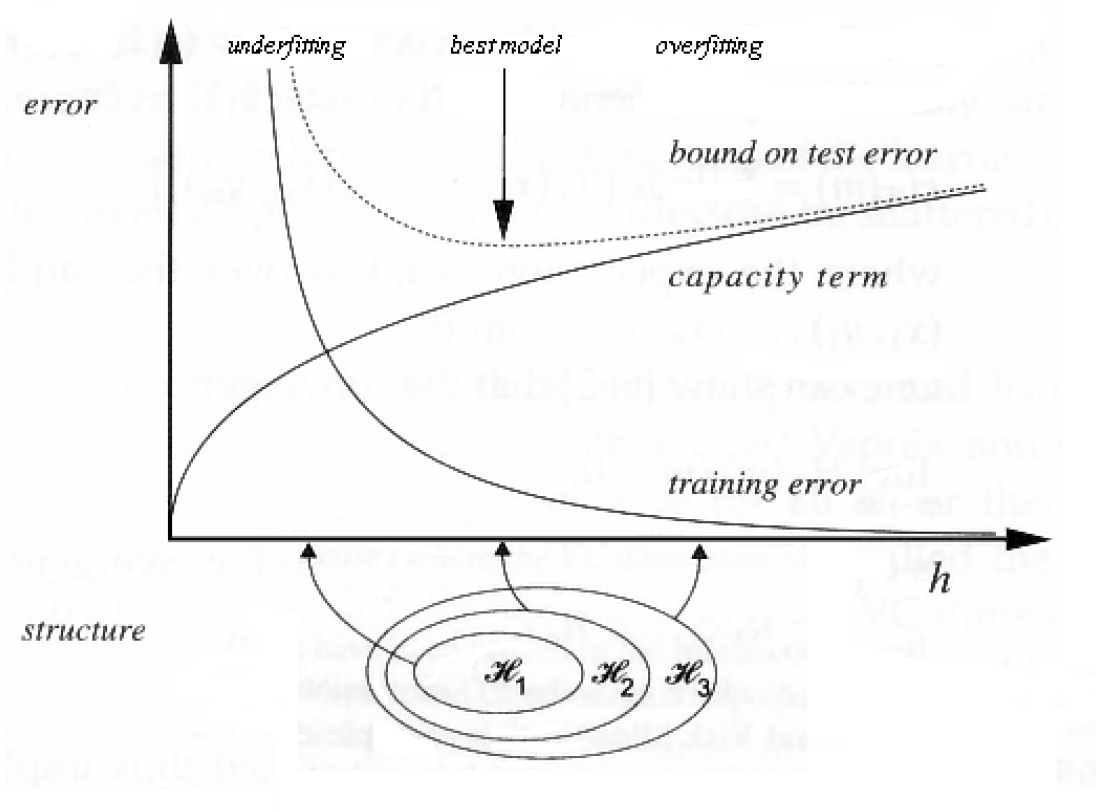
\includegraphics[width=13cm]{Overfitting2.png}

Notre objectif est de trouver ce 'creux', ce minimum, à mi-chemin entre le sous-apprentissage (underfitting) et le sur-apprentissage (overfitting).\\


\subsection{Recherche et évaluation du modèle optimal (classifieur qui minimise le risque réel)}

\subsubsection{Introduction des enjeux}

Nous cherchons ici à \textbf{trouver} le meilleur classifieur, et \textbf{l'évaluer} (savoir si le meilleur classifieur que l'on peut trouver est "bon"). 

Le "bon" classifieur $\hat f_n$ est celui qui minimise le risque réel $R$. Au lieu de choisir "au hasard" une classe $\mathcal{F}$ et minimiser le risque empirique, on va chercher d'autre méthodes d'estimation pour trouver un $\hat f$ plus 'optimal', qui se rapproche plus du minimum du risque 'réel'.\\

Cela passera par la sélection de $\mathcal{F}$ par la fixation d'hyperparamètres, et éventuellement la 'customisation' de la mesure de risque empirique.\\


\subsubsection{Comment se traduit concrètement le choix d'un classifieur}

Pour un type de classifieur (SVM par ex.), on va sélectionner d'éventuels (hyper) paramètres (kernel linéaire par ex.) qui vont déterminer la classe $\mathcal{F}$. Puis suite à la définition de notre mesure du risque empirique, l'algorithme $\mathcal{A}$  va trouver les éventuels paramètres (vecteur $w$ définissant l'hyperplan pour le perceptron par ex.) qui minimisent celui-ci sur l'échantillon d'entraînement $\mathcal{D}_{train}$ donné, ce qui définira au final notre classifieur $\hat f_n$.\\


Les hyper-paramètres sont divers et dépendent du type de classifieur envisagé:

Choix lorsque c'est possible du paramètre de "lissage", qui définit la notion de distance ou qui quantifie l'erreur(fonction de distance en k-nn, choix du paramètre h pour méthode par noyaux SVM, paramètre de fonction Hinge pour perceptron plutôt que "ZeroOneLoss").

Paramètres qui influent sur la complexité de notre classe: profondeur maximum dans un arbre de décision, type de kernel dans une SVM (par exemple degré polynomial dans le cadre d'un kernel polynomial), nombre de couches d'un réseau de neurones, etc. \\

\textbf{Synthèse des choix}
\begin{outline}
\1 Type de classifieur
\1 Eventuels hyper-paramètres
\1 Mesure d'erreur: fonction de coût, et fonction du risque empirique.
\1 Algorithme de minimisation de fonction de risque empirique
\end{outline}
Les éventuels paramètres du classifieur seront ensuite obtenus par l'application de l'algorithme $\mathcal{A}$ sur $\mathcal{D}_{train}$.

\subsubsection{Comment évaluer (et en conséquence choisir) nos classifieurs, autrement qu'en minimisant le risque empirique si cette dernière méthode n'est pas pertinente?}

Comme évoqué aux chapitres précédents, la minimisation du risque empirique a ses limites pour trouver le classifieur optimal dans une classe $\mathcal{F}$ donnée. En effet nous courons le risque de "sur-apprendre" sur notre échantillon d'entraînement. 

Une autre limite, est que nous n'appliquons notre algorithme de minimisation du risque empirique $\mathcal{A}$ qu'à posteriori du choix de la classe $\mathcal{F}$. Ainsi cela ne répond pas à la question de savoir comment choisir ces "hyper"-paramètres.\\

Deux grandes méthodes sont envisageables pour 'noter' un classifieur $\hat f_n$ (résultat de la démarche du choix de la classe $\mathcal{F}$ et de l'application d'un algorithme $\mathcal{A}$ de minimisation d'une mesure de risque empirique $\hat R_n$).
\begin{outline}
\1 Une démarche basée sur la théorie, par pénalisation de la complexité du modèle. Cette méthode essaie d'imaginer comment théoriquement le risque empirique diverge du risque réel selon la complexité de la classe $\mathcal{F}$, et essaie de contrebalancer cette différence.
\1 Des démarches de validation empiriques, en testant la capacité de prédiction de notre classifieur, sur des données auxquelles il n'a pas été confrontées précédemment. L'hypothèse sous-jacente est que l'échantillon de test $\mathcal{D}_{test}$ est composé d'observations issues de la loi de probabilité de $(X,Y)$ (la même que les observations de $\mathcal{D}_{train}$), et permet ainsi d'estimer l'espérance "à priori" (relativement au tirage de $\mathcal{D}_{train}$) de notre risque de prédiction: $\mathbb{E}_{\mathcal{D}_{train}}[R(\hat f_n)] =\mathbb{E}_{\mathcal{D}_{train}}[ \mathbb{E}_P(l(X,Y,\hat f_n(X))|\mathcal{D}_{train})]$.
\end{outline}

Dans les faits, il est très compliqué (et périlleux) d'opter pour la méthode théorique. La validation se fait toujours par validation empirique, et l'on pourra distinguer deux cas selon nos contraintes (computationelles et de volume de données disponibles).\\

\myparagraph{Partage de l'échantillon (apprentissage, validation, test)} 
Lorsque l'on a suffisamment de données, on cherche à partager l'échantillon (apprentissage, validation, test), afin de distinguer l'apprentissage des paramètres de notre classifieur sur $\mathcal{D}_{train}$ et l'apprentissage de nos hyper-paramètres sur $\mathcal{D}_{val}$, et finalement le calcul du risque empirique sur un ensemble d'observations $\mathcal{D}_{test}$ auquel notre procédure d'estimation n'a pas eu accès, et dont les observations sont supposées suivre la loi de probabilité de $(X,Y)$.

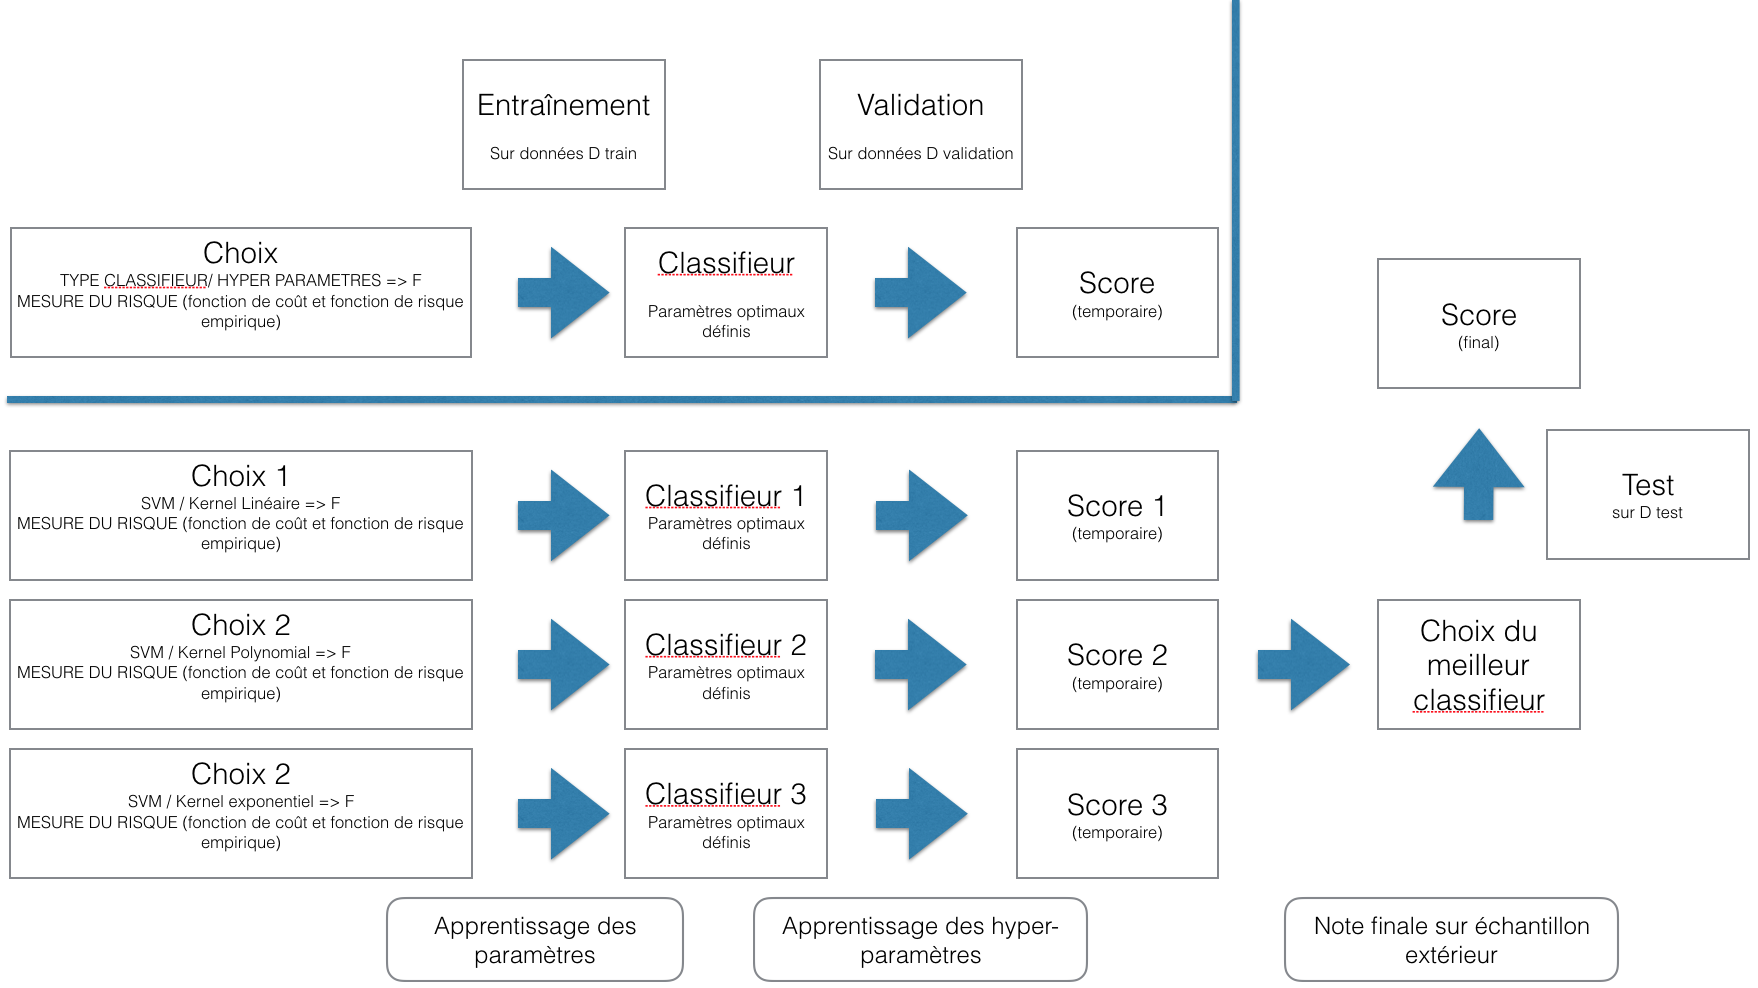
\includegraphics[width=13cm]{Validation.png}

\begin{remark*}
Cette section n'est pas tirée explicitement du cours. C'est une interprétation à prendre avec des pincettes. 
\end{remark*}
\begin{remark*}
Perso: voir si cela est pertinent de définir deux fonctions de risque empirique: une biaisée avec pénalisation pour l'entraînement pour obtenir un "bon" estimateur, une autre "normale" = moyenne empirique, pour la phase finale de test (un peu comme lorsque l'on validait notre LSLasso en regression linéaire avec une mesure d'erreur de prediction non biaisée alors qu'on avait obtenu notre estimateur en introduisant un biais dans l'erreur de prediction à la base). 
\end{remark*}
\myparagraph{Méthode de validation croisée}
\textbf{Idée générale}: itérer l'estimation de l'erreur sur plusieurs échantillons de validation, puis en calculer la moyenne.\\

C'est indispensable pour réduire la variance et améliorer la précision lorsque la taille de l'échantillon initial est trop réduite pour en extraire un échantillon de validation ou test de taille suffisante.\\

\textbf{Méthode}\\
\begin{outline}
\1 Découper aléatoirement l'échantillon $\mathcal{D}_n$ en K parts de taille approximativement égales selon une loi uniforme.
\1 Répéter K fois l'opération qui consiste à mettre de côté l'une des parties, estimer le modèle sur les K-1 parties restantes, calculer l'erreur empirique $\hat R_n(\hat f_n)$ sur chacune des observations n'ayant pas participé à l'estimation.
\1 Moyenner toutes ces erreurs pour aboutir à l'estimation par validation croisée.
\end{outline}

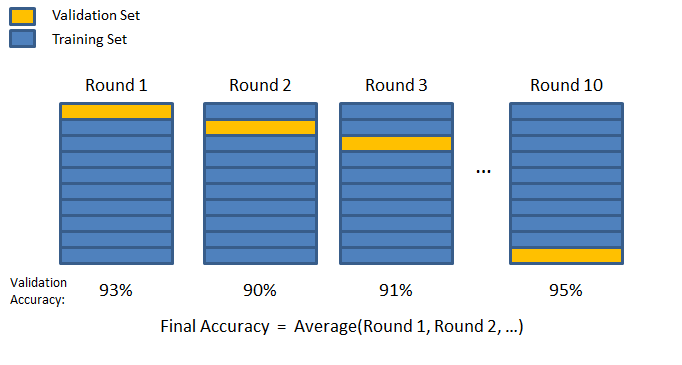
\includegraphics[width=13cm]{CrossValidation.png}

On pourrait imaginer un rééchantillonage par Jackknife ou par Bootstrap.\\
\begin{remark*}
Attention! Il n'y a pas de troisième échantillon pour tester au final. Le but ici n'est pas de tuner nos hyperparamètres, mais de tester la qualité de notre classifieur dont les paramètres ont été entraînés sur $\mathcal{D}_{train}$, pour une classe $\mathcal{F}$ fixée.

\end{remark*}


\myparagraph{Focus sur l'approche par régularisation pour limiter la complexité du modèle}

Une solution pour maîtriser la "variance" du risque 'réel' de notre classifieur est de pénaliser la complexité de notre modèle. Ainsi à la place de minimiser $\hat R_n(f)$, on minimise la somme de deux termes:
\begin{outline}
\1 le risque empirique $$\hat R_n(f, \mathcal{D}_n) = \frac{1}{n}\sum_{i=1}^{n}\mathit{l}(x_i,y_i,f(x_i))$$
\1 et un terme régularisateur qui mesure la complexité de $f$ : $\Omega(f)$
\end{outline}

On cherche au final: $$ \hat f = {\rm arg} \displaystyle\min_{f \in \mathcal{F}} \left( \hat R_n(f, \mathcal{D}_n) + \lambda \Omega(f) \right)$$

NB : on cherche a obtenir un compromis entre une bonne adequation aux donnees et une complexite limitee : $\Omega(f)$ est en
général choisi pour renforcer la régularite de la fonction.\\

\begin{remark*} Ces méthodes s'appuient sur le même principe que les méthode Lasso ou Ridge en regression linéaire. On introduit un biais pour limiter la variance. On pourra utiliser cette mesure du risque pour l'entraînement d'un modèle mais pas pour sa validation! On leur préférera généralement les méthodes de validation empiriques (ie validation croisée et échantillon de test). Pour ne pas surcharger ce document, les différentes méthodes sont décrites en annexe \ref{Detail_penalisation}. 
 \end{remark*}
 





\pagebreak
\section{Détail des classifieurs}

\subsection{Vue d'ensemble}

On distingue deux types d'approches qui seront détaillées dans les chapitres suivants:
\begin{itemize}
\item les approches génératives qui modélisent la distribution de chaque classe individuellement. En ce sens on imaginer pouvoir "générer" des échantillons grâce à notre modèle.
\item les approches discriminantes qui apprennent les frontières (dures, ou douces) entre classes. On cherche donc à discriminer, faire des distinctions entre groupes, sans modelisation des échantillons de chaque classe.
\end{itemize}

Cette page explique plus en détail la différence entre ces deux approches: \url{http://stats.stackexchange.com/questions/12421/generative-vs-discriminative}.

\subsubsection{Les approches dites "génératives"}

Les approches dites "generatives": $f(x) = seuil(\hat P(Y = 1|x))$
et $f$ est fondee sur la modelisation des probabilites conditionnelles de chaque classe: par exemple $P(X=x|Y = -1)$ et $P(X=x|Y = 1)$ dans le cas binaire.

Ces approches cherchent in fine à modéliser les probabilités à posteriori des classes sachant $x$: $P(Y=k|X=x)$


\begin{outline}
\1 Analyse discriminante linéaire (LDA, oui.. c'est bien une générative)
\1 Naive Bayes
\1 Régression logistique linéaire (peut aussi être considérée comme une approche discriminante) 

\end{outline}

\subsubsection{Les approches dites "discriminantes"}

Les approches dites "discriminantes": avec f(x) on essaie de
discriminer entre les classes sans modélisation des probabilités conditionnelles de chaque classe.

\begin{outline}
\1 K plus proches voisins: KNN
\1 Support Vector Machine
\1 Decision Tree
\1 Perceptron

\end{outline}


\subsubsection{Liste des classifieurs détaillés dans ce document}
\begin{itemize}
\item Linear Discriminant Analysis
\item Logistic Regression
\item Perceptron
\item Support Vector Machine
\item K Nearest Neighbors 
\item Decision Tree
\end{itemize}


\subsubsection{Caractérisation des classifieurs}

On va définir pour chaque méthode:

\begin{outline}

\1 Notre espace de représentation des entrées $\mathcal{X}$

\1 Notre espace de représentation des sorties $\mathcal{Y}$

\1 Une classe de fonction $\mathcal{F}$ pour notre classifieur

\1 Une ou plusieurs fonctions $l$ de coût (de scoring) envisageables

\1 Une fonction de risque empirique $\hat R$ cherchant à approcher empririquement $R$, généralement la moyenne empirique des fonctions de coût sur l'ensemble d'apprentissage

\1 Un ou plusieurs algorithmes d'apprentissage, ie de minimisation du risque empirique

\end{outline}

\pagebreak
\subsection{Classifieurs : Linear Discriminant Analysis: LDA}

\subsubsection{Vue d'ensemble}

L'analyse linéaire discriminante est une approche générative (qui modélise la distribution des individus de chaque classe, $P(X=x|Y=k$).\\

On cherche à modeliser:
$$\forall k \in \mathcal{Y}, \forall x \in \mathcal{X} \quad \eta(x)=P(Y=k|X=x)$$


\textbf{Assomptions}\\
Cette méthode se base sur les assomptions suivantes:
\begin{itemize}
\item $P(X|Y=1)$ et $P(X|Y=-1)$ ont des densités supposées gaussiennes de matrice de coviariance égales.
\item $P(Y=1)$ et $P(Y=-1)$ sont supposées connues (probabilités à priori des classes).
\end{itemize}


\textbf{Esprit général}\\

Soit $f_{LDA}$ le classifieur, alors, sa définition de base est:
\begin{equation}
f_{LDA}=
\left\lbrace
\begin{array}{ccc}
1  & \mbox{si} & log(\frac{P(Y=1|X=x)}{P(Y=-1|X=x)})>0 \quad \mbox{ie}, P(Y=1|X=x)>P(Y=-1|X=x)\\
-1 & \mbox{sinon}
\end{array}\right.
\end{equation}
Ou plus simplement:
$$f_{LDA} : x \rightarrow sign(\hat g(x)) \quad avec \quad \hat g(x):= log(\frac{\hat P(Y=1|X=x)}{\hat P(Y=-1|X=x)}) $$
Voire, sous une version 'maximum de vraissemblance':
$$f_{LDA}(x) = argmax_{k \in \{-1,1\}} \hat P(Y=k|X=x) $$

Ce qui se traduit par: la probabilité de $Y=1$ sachant $X=x$ and plus grande que la probabilité de $Y=-1$ sachant $X=x$, alors je prédit que $Y=1$. Dans le cas contraire je prédis: $Y=-1$. Ce qui semble assez logique.\\

Cela correspond au final au classifieur de Bayes avec un espace $\mathcal{Y}$ à deux classes:
$$f_{Bayes}(x) = {\rm arg} \displaystyle\max_{y \in \mathcal{Y}} P(Y=y|X=x)$$


\subsubsection{Implémentation}

On ne connait évidemment, malheureusement pas $P(Y=1|X=x)$, et $P(Y=-1|X=x)$, c'est à dire la probabilité que la classe soit égale à $y$ sachant les caractéristiques $x$ de l'individu. C'est le problème que nous cherchons à résoudre.\\


En revanche, ce que l'on est sensé savoir, et les assomptions faites pour appliquer cette méthode, nous donnent: 
\begin{itemize}
\item les probabilités à priori $P(Y=1)$ et $P(Y=-1)$ des classes (que nous supposons connues)
\item $P(X|Y=1)$ et $P(X|Y=-1)$ ont des densités gaussiennes de matrice de coviariance égales (assomption).
\item nous disposons d'un échantillon $\mathcal{D}_n$ labelisé nous permettant d'estimer la moyenne et la variance de nos vecteurs aléatoires $(X|Y=1)$ et $(X|Y=-1)$ (méthode d'estimation paramétrique, basée sur l'assomption gaussienne). Au final nous modélisons $P(X|Y=1)$ et $P(X|Y=-1)$, ce qui constitue le coeur de l'approche générative.
\end{itemize}

Ainsi nous pouvons estimer $P(Y=1|X=x)$, et $P(Y=-1|X=x)$ en se basant sur la formule de Bayes:
$$\forall k \in \mathcal{Y}, \forall x \in \mathcal{X}, \quad P(Y=k|X=x) = \frac{ P(X=x|Y=k) \times P(Y=k)}{P(X=x)} $$
$$\forall k \in \mathcal{Y}, \forall x \in \mathcal{X}, \quad P(Y=k|X=x) = \frac{ P(X=x|Y=k) \times P(Y=k)}{\sum_{l \in \mathcal{Y}} P(X=x|Y=l)\times P(Y=l)} $$

Dont nous pouvons estimer tous les termes avec les estimateurs suivants:\\
\begin{itemize}
\item $\hat P(Y=k)$ sera calculé à partir de la proportion de chaque classe dans l'ensemble d'apprentissage $\mathcal{D}_n$
\item $\hat P(X=x|Y=k)$ sera détaillé dans la partie suivante
\item $\hat P(X=x) = \sum_{l \in \mathcal{Y}} \hat P(X=x|Y=l)\times \hat P(Y=l)$ est une fonction des deux premiers termes ci-dessus.
\end{itemize}


\textbf{Estimation des paramètres des lois de $(X|Y=1)$ et $(X|Y=-1)$: $\hat \mu_1, \hat \mu_{-1}, \hat \Sigma$, pour obtenir $\hat P(X=x|Y=k)$:}\\

$(X|Y=1)$ et $(X|Y=-1)$ sont deux vecteurs aléatoires dont nous supposons qu'ils sont issus de gaussiennes multivariées de même matrice de covariance.

Pour déterminer une gaussienne multivariée il suffit de déterminer deux paramètres: $\mu$ son vecteur d'esperance, et $\Sigma$ sa matrice de covariance.\\

En l'occurence, il faut diviser notre échantillon d'apprentissage $\mathcal{D}_n$ en deux échantillons distincts: 
\begin{itemize}
\item $\mathcal{D}_1 = \{(x_i,y_i) \in \mathcal{D}_n, \quad y_i=1 \}$ 
\item $\mathcal{D}_{-1} = \{(x_i,y_i) \in \mathcal{D}_n, \quad y_i=-1 \}$
\end{itemize}

A partir de ces deux échantillons nous pouvons estimer leurs vecteurs d'esperance respectifs $\mu_1$ et $\mu_{-1}$ à partir de leurs moyennes empiriques:
\begin{itemize}
\item esperance de $X$ dans la classe 1, $(X|y=1)$, $\hat \mu_1 = \frac{1}{|{D}_1|} \sum_{x_i \in \mathcal{D}_1} x_i$
\item esperance de $X$ dans la classe -1, $(X|y=-1)$, $\hat \mu_{-1} = \frac{1}{|{D}_{-1}|} \sum_{x_i \in \mathcal{D}_{-1}}  x_i$
\end{itemize}

Je ne détaille pas ici la méthode pour obtenir $\hat \Sigma$, mais faisons l'hypothèse que nous l'ayons obtenu.
A vrai dire l'estimation de la matrice de covariance $\Sigma$ est un problème souvent complexe à résoudre, qui se résout généralement par maximisation de la vraisemblance.\\

Au final nous pourrons obtenir une estimation de $P(X=x|Y=k)$ en appliquant la densité d'une gaussienne multivariée de paramètres $(\hat \mu_k,\hat \Sigma)$: 
$$\hat P(X=x|Y=k)= \frac{1}{ (2 \pi)^n |\hat \Sigma_k|^{1/2} } \exp \left( \frac{1}{2}(x- \hat \mu_k)^T \hat \Sigma_k^{-1}(x-\hat \mu_k) \right) $$

\textbf{Formulation du classifieur  $f_{LDA}$ et de $\hat g(x)$}\\

Avec le résultat de la section précédente, et en reprenant la formulation de $\hat g(x)$, on peut réduire $\hat g(x)$ sous la forme suivante:
$$\hat g(x) = log(\frac{\hat P(Y=1|X=x)}{\hat P(Y=-1|X=x)}) = \hat \theta_0 + \hat \theta^T x$$
avec $\hat \theta_0$ et $\hat \theta$ des fonctions de $\hat \mu_1, \hat \mu_{-1}, \hat \Sigma$ et $\hat P(Y=1)$ : 
$$ \hat \theta_0 = log(\frac{\hat P(Y=1)}{\hat P(Y=-1)}) -\frac{1}{2}(\hat \mu_1 + \hat \mu_{-1})^T \hat \Sigma^{-1}(\hat \mu_1 - \hat \mu_{-1})$$
$$ \hat \theta = (\hat \mu_1 - \hat \mu_{-1})^T \hat \Sigma^{-1}$$

Si la formule du classifieur $\hat g(x) = \hat \theta_0 + \hat \theta^T x$ est effectivement exactement de la même forme que celle de la régression logistique, la différence fondamentale réside dans la manière de calculer les coefficients $\hat \theta$ et $\hat \theta_0$. Pour plus de détails une explication plus détaillée est en page 127 du livre 'The elements of statistical learning'.

\subsubsection{Synthèse:}

\begin{outline}

\1 Notre espace de représentation des entrées $\mathcal{X} = \mathbb{R}^p$

\1 Notre espace de représentation des sorties $\mathcal{Y}=\{-1,1\}$

\1 Assomptions de base:
\2 $P(X|Y=1)$ et $P(X|Y=-1)$ ont des densités supposées gaussiennes de matrice de coviariance égales.
\2 $P(Y=1)$ et $P(Y=-1)$ sont supposées connus (probabilités à priori des classes).

\1 Classifieur $f$: 
$$f : x \rightarrow sign(\hat g(x)) \quad avec \quad \hat g(x):= log(\frac{\hat P(Y=1|X=x)}{\hat P(Y=-1|X=x)})$$ 
où les estimations de probabilités conditionnelles sont obtenues en se basant sur une hypothèse de lois gaussiennes pour les $X|Y=k$.


\1 Une ou plusieurs fonctions $l$ de coût (de scoring) envisageables (A FAIRE):
\2 Attention, ces fonctions s'appliquent sur $\hat g$, et non pas directement sur le classifieur $\hat f$!
\2 le pourcentage d’erreur : $ZeroOneLoss(x, g(x),y) = |y-sign(g(x))|/2$


\1 Une éventuelle fonction de risque empirique $\hat R$ cherchant à approcher empririquement $R$. Ici nous prenons la moyenne empirique: (attention encore au g à la place du f):
$$\hat R_n(f, \mathcal{D}_n) = \frac{1}{n}\sum_{i=1}^{n}\mathit{l}(x_i,y_i,g(x_i))$$

\1 Pas d'algorithme de minimisation du risque empirique: à la place il y a eu une phase d'estimation pour déterminer les paramètres de nos gaussiennes. Le calcul de l'estimation de la matrice de covariance fait en revanche l'objet d'un algorithme de maximisation de la vraissemblance. C'est en cela qu'il y a apprentissage.

\end{outline}

\subsubsection{Pour aller plus loin, et en pratique}
\url{http://scikit-learn.org/stable/modules/lda_qda.html}

Pour aller plus loin, concernant la différence entre LDA et régression logistique: p127 de 'The elements of statistical learning'.\\

On peut approfondir le sujet en abordant les pistes suivantes:
\begin{itemize}
\item QDA: pour Quadratic Discriminant Analysis: dans ce cas les matrices de covariance de loi de probabilités à posteriori des classes ne sont pas supposées égales: ie on définit $\hat \Sigma_1$ et $\hat \Sigma_{-1}$, au lieu de $\hat \Sigma$
\item la notion de pénalisation: pour améliorer l'estimation des matrices de covariance dans le cas où il y a peu d'individus par rapport au nombre de features considérées.
\end{itemize}

A noter que cette méthode est très proche de la regression logistique. Cependant la regression logistique est généralement préférée car faisant moins d'assomptions (par exemple sur les loi des $X|Y=k$).\\
Par ailleurs la regression logistique est plus robuste aux valeurs aberrantes.\\

Le principe est également très proche de la méthode Gaussian Naive Bayes.
Une différence est que de manière générale, les méthodes dites 'bayesiennes naïves' font comme assomption l'indépendance entre variables explicatives. La méthode "Gaussian Naive Bayes" fait donc d'indépendance en plus de l'hypothèse de normalité (ce qui donne des matrices de covariances diagonales). 

\pagebreak
\subsection{Classifieurs : régression logistique}

\subsubsection{Vue d'ensemble}

La regression logistique peut être considérée comme une approche générative (qui modélise la distribution des individus de chaque classe, $P(X=x|Y=k$).\\ 
On cherche à modeliser:
$$\forall k \in \mathcal{Y}, \forall x \in \mathcal{X} \quad \eta(x)=P(Y=k|X=x)$$

Cependant elle peut également être considérée comme une analyse discriminante qui cherche à séparer au mieux des classes en maximisant un critère de performance. C'est cette vision qui est majoritaire.\\

Cette méthode est ainsi souvent nommée semi-paramétrique, du fait de sa dualité.\\

\url{https://www.quora.com/What-is-the-difference-between-logistic-regression-and-discriminant-analysis}\\

\url{https://en.wikipedia.org/wiki/Discriminative_model}\\

\subsubsection{Forme du problème}
On se basera ici dans un cadre binaire avec comme classes 0 et 1.\\
On définit un classifieur tel que:
$$
f_{Rlog}=
\left\lbrace
\begin{array}{ccc}
1  & \mbox{si} & log(\frac{P(Y=1|X=x)}{P(Y=0|X=x)})>0 \quad \mbox{ie}, P(Y=1|X=x)>P(Y=0|X=x)\\
0 & \mbox{sinon}
\end{array}\right.
$$

\textbf{Modèle}\\
Le modèle de la régression logistique se base sur l'hypothèse suivante:
$$\exists (\theta_0,\theta) \in (\mathbb{R},\mathbb{R}^p), \quad log(\frac{P(Y=1|X=x)}{P(Y=0|X=x)}) = \theta_0 + \theta^T x$$

Cette hypothèse fait penser à une hypothèse de normalité sur la loi de $(X|Y)$ (voir détail de LDA), en réalité, l'assomption est moins forte qu'en LDA.\\

La forme rappelle évidement également le régressions linéaires.\\

Expliquer plus en détail les différences: maximisation de log vraissemblance, en opposition à minimisation du risque quadratique en regression linéaire, à faire.\\

Le modèle de régression logistique provient d'une volonté de modéliser les probabilité à posteriori des classes par des fonctions linéaire des vecteurs x, tout en s'assurant que la somme des probabilités soit égale à 1.

p119 - 'The elements of statistical learning'\\

\textbf{Conséquences}\\

On prouve facilement en passant à l'exponentielle que:

$$P(Y=1|X=x) = \frac{exp(\theta_0 + \theta^T x)}{1 + exp(\theta_0 + \theta^T x)}$$
$$P(Y=0|X=x) = \frac{1}{1 + exp(\theta_0 + \theta^T x)}$$

Si l'on arrive à estimer $\theta_0$ et $\theta$ par  $\hat \theta_0$ et $\hat \theta$ on obtiendra directement une estimation des probabilités à posteriori des classes:

$$\hat P(Y=1|X=x) = \frac{exp(\hat \theta_0 + \hat \theta^T x)}{1 + exp(\hat \theta_0 + \hat \theta^T x)}$$
$$\hat P(Y=0|X=x) = \frac{1}{1 + exp(\hat \theta_0 + \hat \theta^T x)}$$


On remarque aussi au passage que :
$$ \sum_{k \in \{0,1\}} P(Y=k|X=x) = 1 $$

Cette propriété assure une certaine cohérence à notre modèle. \\

Pour insister sur le fait que la probabilité dépende de $\theta$, nous noterons désormais: $P(Y=k|X=x) = P(Y=k|X=x, \theta)=  p_k(x,\theta) $\\

\textbf{Estimation: ie apprentissage de notre classifieur}\\


\textbf{Solution 1: moindre carrés}\\
A FAIRE\\

\textbf{Solution 2: maximum de vraisemblance}\\

Les régressions logistiques sont généralement entraînées par la méthode d'estimation consistant à maximiser la log-vraisemblance, que nous noterons ici $l(\theta)$ :

$$ l(\theta) = \sum_{i=1}^n log\left(  P(Y=y_i|X=x_i, \theta)\right) $$
$$ l(\theta) = \sum_{i=1}^n \sum_{k \in \{0,1\}}\mathds{1}_{y_i=k} log\left(  P(Y=k|X=x_i, \theta)\right) $$

$x_i$ et $y_i$ étant respectivement les valeur des variables explicatives, et la classe, d'un individu.

En utilisant nos resultats précédents nous pouvons prouver que:
$$ l(\theta) = \sum_{i=1}^n log(1 + exp(-u_i (\theta_0 + \theta^T x))) $$
avec $u_i = 2 \times \mathds{1}_{y_i=0}-1$ \\

Nous cherchons ainsi à résoudre le problème convexe suivant:
$$ (\hat \theta_0,\hat \theta)\in argmax_{(\theta_0, \theta)\in(\mathbb{R},\mathbb{R}^p)} l(\theta_0,\theta)$$ 

Le problème est généralement résolu par la méthode de Newton, on pourrait utiliser une simple descente de gradient.

\subsubsection{Synthèse}
\begin{outline}

\1 Notre espace de représentation des entrées $\mathcal{X} = \mathbb{R}^p$

\1 Notre espace de représentation des sorties $\mathcal{Y}=\{0,1\}$

\1 Assomption de base:
$$\exists (\theta_0,\theta) \in (\mathbb{R},\mathbb{R}^p), \quad log(\frac{P(Y=1|X=x)}{P(Y=0|X=x)}) = \theta_0 + \theta^T x$$

\1 Une classe de fonction $\mathcal{F}$ pour notre classifieur: 
$$F = \left\{ 
f_{Rlog}(x,\theta_0,\theta)=
\left\lbrace
\begin{array}{ccc}
1  & \mbox{si} & log(\frac{P(Y=1|X=x)}{P(Y=0|X=x)}) = \theta_0 + \theta^T x >0 \\
0 & \mbox{sinon}
\end{array}\right. 
(\theta_0,\theta) \in (\mathbb{R},\mathbb{R}^p)
\right\}$$
Au final similaire à la famille de classifieurs du perceptron.

\1 Une ou plusieurs fonctions $l$ de coût (de scoring) envisageables (A FAIRE):


\1 Une éventuelle fonction de risque empirique $\hat R$ cherchant à approcher empririquement $R$. Ici nous prenons la moyenne empirique: (attention encore au g à la place du f):
$$\hat R_n(f, \mathcal{D}_n) = \frac{1}{n}\sum_{i=1}^{n}\mathit{l}(x_i,y_i,g(x_i))$$

\1 Plusieurs algorithmes possibles pour résoudre le problème d'apprentissage: A FINIR

\subsubsection{Pour aller plus loin}
\url{http://stats.stackexchange.com/questions/162257/whats-the-difference-between-logistic-regression-and-perceptron}\\

\url{http://scikit-learn.org/stable/modules/linear_model.html#logistic-regression}

\end{outline}

\pagebreak
\subsection{Classifieurs linéaires affines : Perceptron}

\textbf{Classe de fonction pour notre classifieur}\\

Un classifieur linéaire est un classifieur qui associe à chaque observation $x$ une étiquette dans $\mathcal{Y}$ (ici $\mathcal{Y} = \{-1,1\}$) selon sa position par rapport à un hyperplan affine. \\

Chaque classifieur linéaire est donc lié à
un hyperplan (affine) de $R^p$ que l’on définit pour un certain vecteur directeur (aussi dit vecteur normal)
$w = (w_0,,,w_p)^ \in \mathbb{R}^{p+1}$ par
$$H_w = \left\{ x\in R^p : \hat g_w(x):=w_0 + \sum_{i=1}^{p}w_ix_i =0 \right\}$$

Pour classer une observation $x$ (i.e., affecter une étiquette -1 ou 1) on utilise alors $sign(\hat g_w(x))$.

Ainsi, la fonction $x \rightarrow sign(\hat g_w(x))$ est le classifieur binaire de frontière linéaire (affine) définie par $w$.

L’objectif du perceptron est de trouver un hyperplan qui sépare le mieux possible les données en deux groupes. On aimerait donc que de chaque côté de l’hyperplan séparateur, les étiquettes soient le plus
possible homogènes. 

Le vecteur $w$ est appelé vecteur de poids. Le coefficient $w_0$ est l’ordonnée à l’origine (intercept en anglais).\\

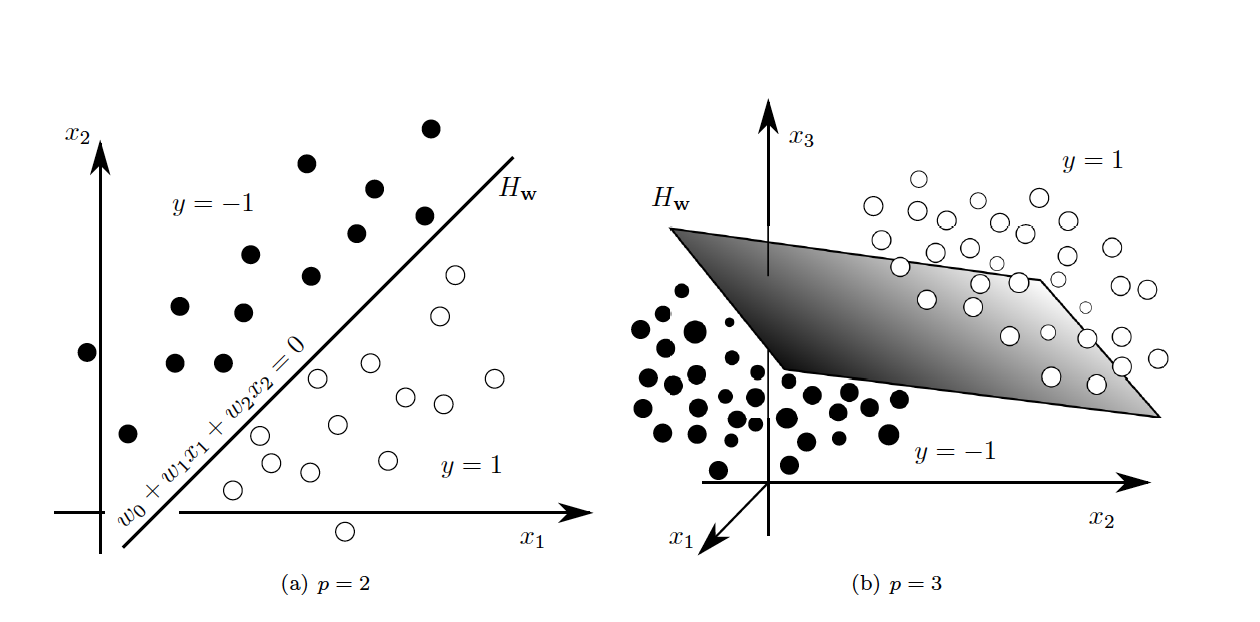
\includegraphics[width=13cm]{Perceptron.png}

Figure 1 – Exemple de séparation de classe (1 pour les points blanc, 1 pour les noirs) par des hyperplans
affines, en dimension p = 2 et p = 3

\textbf{Fonction de coût}\\

Le coût que l’on veut minimiser (en fonction de $w$) est $ E $
, l’espérance de la fonction de perte sur l’ensemble des données. Trois fonctions de perte sont utilisées habituellement et définies ci-dessous:
\begin{outline}
\1 le pourcentage d’erreur : $ZeroOneLoss(x,f(x),y) = |y-sign(f(x))|/2$
\1 l’erreur quadratique : $MSELoss(x,f(x),y) = (y -f(x))^2$
\1 l’erreur hinge (i.e., charnière en français) : $HingeLoss(x,f(x),y) = max(0,1-y.f(x))$ 
\end{outline}

\textbf{Algorithme de descente de gradient stochastique}\\

Dans le cas général, il est bien sûr impossible de faire une recherche exhaustive de l’espace $\mathbb{R}^{p+1}$ où
évolue $w$ afin de trouver le coût minimum. De plus on ne peut pas observer $R(f) = \mathbb{E}_P(l(X,Y,f(X))) $ , on peut donc
seulement tenter de minimiser sa contrepartie empirique :
$$\hat R_n(f, \mathcal{D}_n) = \frac{1}{n}\sum_{i=1}^{n}\mathit{l}(x_i,y_i,f(x_i))$$
La méthode du perceptron consiste à utiliser une variante de l’algorithme de descente du gradient, une méthode usuelle et générale d’optimisation de fonction différentiable. La méthode de descente de gradient est itérative : à chaque étape, le poids courant est corrigé dans la direction du gradient, mais en
sens opposé. 

L’algorithme converge dans le cas général vers un minimum local pour peu que le pas soit bien choisi. De plus, le minimum atteint est global pour les fonctions convexes.

La méthode du gradient stochastique est une variante qui propose de ne pas utiliser le gradient complet, qui requiert de calculer une somme sur les n observations, mais plutôt de tirer (aléatoirement ... ou non) un couple $(x_i, y_i)$ sur laquelle on calcul un gradient. On peut aussi montrer que cet algorithme
converge sous certaines conditions cf. [SSBD14, page 157] ou [Bot98].

L’algorithme du perceptron est décrit de la manière suivante :\\



\begin{algorithm}[H]
 \KwData{les observations et leurs étiquettes $\mathcal{D}_n = f(x_i, y_i) $ le pas de gradient $\epsilon$ ;
le nombre maximal d’itérations : $n_{iter}$ ;}
 \KwResult{$w$}
 initialiser (aléatoirement) $w$; initialiser $j = 0$\
 
 \While{$j \neq n_{iter}$}{
  $w \leftarrow w$\;
  \For{$i = 1$ to $n$}{
   $w \leftarrow w - \epsilon \nabla_w l(x_i,\hat f(x_i),y_i) $
   \;
   }{
   $j \leftarrow j +1$ \;
  }
 }
 \caption{Perceptron (version cyclique)}

\end{algorithm}

Remarque La méthode du gradient stochastique est aussi disponible dans sklearn sous le nom SGDClassifier (SGD est l’abréviation Stochastic Gradient Descent). Une description est donnée sur
la page : http://scikit-learn.org/stable/modules/sgd.html.\\

\textbf{Synthèse:}

\begin{outline}

\1 Notre espace de représentation des entrées $\mathcal{X} = \mathbb{R}^p$

\1 Notre espace de représentation des sorties $\mathcal{Y}=\{-1,1\}$

\1 Une classe de fonction $\mathcal{F}$ pour notre classifieur: $$F = \left\{ f_w : x \rightarrow sign(\hat g_w(x)) \quad avec \quad \hat g_w(x)=w_0 + \sum_{i=1}^{p}w_ix_i \quad, \quad w \in \mathbb{R}^p \right\}$$


\1 Une ou plusieurs fonctions $l$ de coût (de scoring) envisageables:
\2 Attention, ces fonctions s'appliquent sur $\hat g$, et non pas directement sur le classifieur $\hat f$!
\2 le pourcentage d’erreur : $ZeroOneLoss(x, g(x),y) = |y-sign(g(x))|/2$
\2 l’erreur quadratique : $MSELoss(x,g(x),y) = (y -g(x))^2$
\2 l’erreur hinge (i.e., charnière en français) : $HingeLoss(x,g(x),y) = max(0,1-y.g(x))$

\1 Une fonction de risque empirique $\hat R$ cherchant à approcher empririquement $R$. Ici nous prenons la moyenne empirique: (attention encore au g à la place du f):
$$\hat R_n(f, \mathcal{D}_n) = \frac{1}{n}\sum_{i=1}^{n}\mathit{l}(x_i,y_i,g(x_i))$$

\1 Un ou plusieurs algorithmes d'apprentissage, ie de minimisation du risque empirique:
\2 Algorithme de descente de gradient (déconseillé)
\2 Algorithme de descente par coordonnées (meilleur)

\end{outline}

\pagebreak
\subsection{Classifieur: k plus proches voisins}
\textbf{Approche intuitive}

L’algorithme des k-plus proches voisins (k-nn : pour k-nearest neighbors en anglais) est un algorithme
intuitif, aisément paramétrable pour traiter un problème de classification avec un nombre quelconque
d’étiquettes.
Le principe de l’algorithme est particulièrement simple : pour chaque nouveau point x on commence
par déterminer l’ensemble de ses k-plus proches voisins parmi les points d’apprentissage que l’on note
$V_k(x)$ (bien sûr on doit choisir $1 \leq k \leq n$ pour que cela ait un sens). La classe que l’on affecte au nouveau point x est alors la classe majoritaire dans l’ensemble $V_k(x)$. Une illustration de la méthode est donnée en Figure 1 pour le cas de trois classes.

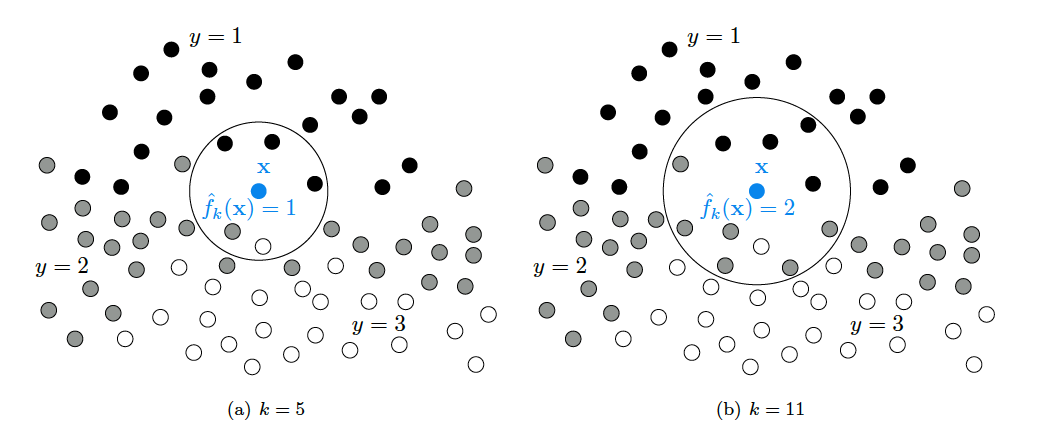
\includegraphics[width=13cm]{Knn.png}

Figure 1 – Exemple de fonctionnement de la méthode des k-plus proches voisins pour des valeurs du
paramètres k = 5 et k = 11. On considère trois classes, L = 3, représentées respectivement en noir
(y = 1), en gris (y = 2) et en blanc (y = 3).\\

\textbf{Approche formelle}

Approche formelle
Pour définir précisément la méthode, il faut commencer par choisir une distance $d : \mathbb{R}^p \times \mathbb{R}^p \rightarrow \mathbb{R}$
Pour un nouveau point $x_{new}$, on définit alors l’ensemble de ses k-plus proches voisins $V_k(x_{new})$ au sens de cette distance. On peut procéder de la manière suivante : pour chaque $x_{new} \in \mathbb{R}^p$ et pour chaque $i = 1 .... n$,
on note $d_i(x_{new})$ la distance entre $x_{new}$ et $x_i$ : $d_i(x_{new}) = d(x_i; x_{new})$ . On définit la première statistique de rang $r_1(x_{new})$ comme l’indice du plus proche voisin de $x_{new}$ parmi $x_1,....,x_n$, c’est-à-dire:
$$ r_1(x_{new}) = i^{\ast} \Leftrightarrow d_{i^{\ast}}(x)_{new} = \min_{1\leq i \leq n} d_i(x_{new})$$


Remarque 1. S’il y a plusieurs candidats pour la minimisation ci-dessus, on ordonne les ex-æquos de manière arbitraire (généralement aléatoirement).\\

Par récurrence on peut ainsi définir le rang $r_k(x_{new})$ pour tout entier $1 \leq k \leq n $:

$$r_k(x_{new}) = i^{\ast} \Leftrightarrow d_i^{\ast}(x_{new}) = \min_{\substack{ 1\leq i \leq n \\ i\neq r_1,...,r_{k-1}}} d_i(x_{new}) $$

L’ensemble de k-plus proches voisins de $x$ s’exprime alors par $V_k(x_{new}) = \{x_{r_1},..,x_{r_k}\}$. 

Pour finir, la décision pour classifier le point $x$ se fait par vote majoritaire, en résolvant le problème suivant :
$$\hat f_k(x_{new}) \in \underset{y \in \mathcal{Y}}{\arg\max} \left( \sum_{j=1}^{k}\mathds{1}_{\{y_{r_j}=y\}}  \right)$$

Le module sklearn.neighbors de scikit-learn, (cf. http://scikit-learn.org/stable/modules/
neighbors.html) implémente les méthodes de classification et régression à base de k-plus proches voisins.\\

Une variante possible très utilisée consiste à pondérer les poids du $j_{eme}$ voisin selon $\exp^{-d^2_j/h}$ ($h$ contrôlant le niveau de pondération) : cela revient à choisir comme classifieur par : 
$$\hat f_k(x_{new}) \in \underset{y \in \mathcal{Y}}{\arg\max} \left( \sum_{j=1}^{k}\exp(-d^2_j/h) \mathds{1}_{\{y_{r_j}=y\}}  \right)$$




Des détails généraux sur la méthode des k-plus proches voisins se trouvent dans [HTF09, Chapitre 13].
Pour améliorer la compréhension théorique de la méthode on peut se reporter au livre [DGL96, Chapitre
11] et les limites de la méthode quand k = 1 http://certis.enpc.fr/%7Edalalyan/Download/DM1.pdf.

Enfin pour les considérations algorithmiques on pourra commencer par lire http://scikit-learn.org/
stable/modules/neighbors.html brute-force.\\

\textbf{Synthèse}\\

\begin{outline}

\1 Notre espace de représentation des entrées $\mathcal{X} = \mathbb{R}^p$

\1 Notre espace de représentation des sorties $\mathcal{Y}=\{1,...,L\}$

\1 Une classe de fonction $\mathcal{F}$ pour notre classifieur: 
$$F = \left\{\hat f_k(x_{new}) \in \underset{y \in \mathcal{Y}}{\arg\max} \left( \sum_{j=1}^{k}\exp(-d^2_j/h) \mathds{1}_{\{y_{r_j}=y\}}  \right), d \in \mathcal{D}, h \in \mathbb{R}\right\}$$
\2 Dans ce cas, cela implique le choix d'une fonction $d$ de distance appartenant à une classe $\mathcal{D}$ à définir. Dans le cas le plus simple: $d(x,y)$ représente la distance euclidienne $||x-y||_2$
\2 Cela nécessite le choix d'un $h$, régulant l'impact de la distance dans le vote à la majorité.

\1 Une fonctions $l$ de coût très simple: $l(x, f(x),y) = \mathds{1}_{\{f(x)\neq y\}} $

\1 Une fonction de risque empirique $\hat R$ cherchant à approcher empririquement $R$. Ici nous prenons la moyenne empirique:
$$\hat R_n(f, \mathcal{D}_n) = \frac{1}{n}\sum_{i=1}^{n}\mathit{l}(x_i,y_i,f(x_i))$$

\1 L'algorithme est très simple, on réalise un seul passage de calcul pour obtenir une classification d'une observation.


\end{outline}

\pagebreak
\subsection{Classifieurs : SVM, support vector machine : en cours}

Les SVM ont été introduites par Vapnik, et sont abordées au chapitre 12 du livre [1]. La popularité
des méthodes SVM, pour la classification binaire en particulier, provient du fait qu’elles reposent sur l’application
d’algorithmes de recherche de règles de décision linéaires ("hyperplan séparateur"), la recherche
s’effectuant toutefois dans un espace ("feature space") de très grande dimension, lequel est l’image de
l’espace d’entrée original par une transformation  non linéaire.\\

\textbf{Cas simple}\\

\begin{outline}

\1 Cadre statistique.

\1 Classifieurs linéaires de: séparateurs linéaires de marge optimale.

\1 Passage à un classifieur linéaire: SVM

\1 SVR: régression.
\end{outline}
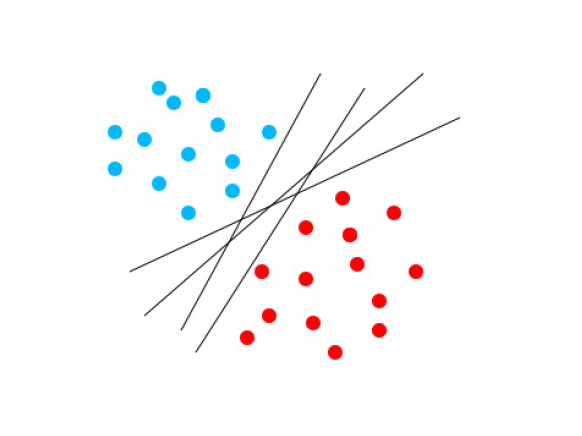
\includegraphics[width=8cm]{SVM1.png}

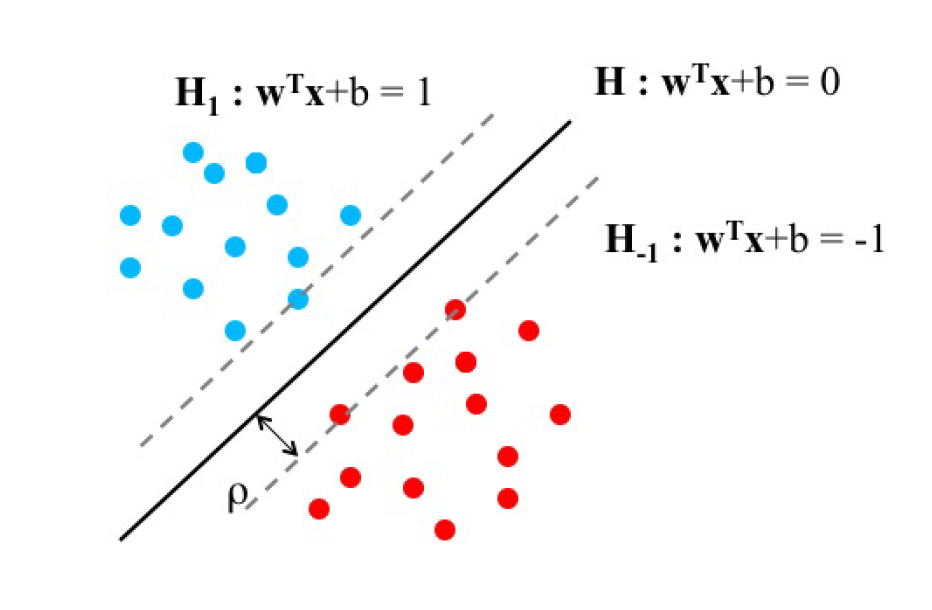
\includegraphics[width=8cm]{SVM2.png}

On veut H0, H1 et H-1 tel que la marge géométrique entre les données et H soit maximale, sous contrainte:\\
- les données 'noires' soient au dessus de H1, \\
- les données 'rouges' soient au dessous de H-1.

$$H: \quad w^Tx+b=0$$
$$H_1: \quad w^Tx+b=1$$
$$H_{-1}: \quad w^Tx+b=-1$$

(1)$$ (x^+-x^-) = \lambda w $$
(2)$$ x^+ \in H_+ \quad w^T x_+ + b=1$$
(3)$$ x^- \in H_- \quad w^T x_- + b=-1$$
(2)-(3) $$w^T(x_+-x_-)=2 $$

$$l(y,y')$$

\textbf{Synthèse}\\

\begin{outline}

\1 Notre espace de représentation des entrées $\mathcal{X} = \mathbb{R}^p$

\1 Notre espace de représentation des sorties $\mathcal{Y}=\{-1,1\}$

\1 Une classe de fonction $\mathcal{F}$ pour notre classifieur: 
$$F = $$


\1 Une fonctions $l$ de coût très simple: $l(x, f(x),y) = \mathds{1}_{\{f(x)\neq y\}} $

\1 Une fonction de risque empirique $\hat R$ cherchant à approcher empririquement $R$. Ici nous prenons la moyenne empirique:
$$\hat R_n(f, \mathcal{D}_n) = \frac{1}{n}\sum_{i=1}^{n}\mathit{l}(x_i,y_i,f(x_i))$$

\1 L'algorithme ///.

\end{outline}






\pagebreak
\subsection{Classifieurs : arbre de décision}

\subsubsection{Cadre et notations}
On se place dans le cadre de la classification multi-classe, avec les notations habituelles, on suppose
que les données peuvent être reparties dans K classes. L’ensemble d’apprentissage est de taille n: $\mathcal{D}_n = \{(x_i,y_i), i=1,...,n\}$ contenant les n observations. Pour mémoire
$x_i = (x_1, ..., x_p)^T \in \mathcal{X}   \subset \mathbb{R}^p$ est une observation, et dans le cas bidimensionnel p = 2.

\subsubsection{Algorithme CART: Classification and Regression Trees}

Nous ne considèrerons que des arbres binaires par simplicité : un noeud ne peut avoir que deux enfants, sauf si c’est une feuille, auquel cas il n’en a
aucun.\\

On associe à toute partition des données une représentation par arbre. Au départ l’arbre est restreint à
un seul noeud, sa racine, qui représente l’espace X tout entier. Récursivement, à chaque étape on choisit :
\begin{itemize}
\item une variable $j \in \{1,...,p\}$ (parmi les p possibles), 
\item un seuil: $\tau \in \mathbb{R}$ 
\end{itemize}

 
et l’on partitionne l’espace des variables explicatives en deux sous-ensembles qui sont représentés par deux noeuds dans l’arbre 

$$G(j,\tau) = \{ x= (x_1,...,x_p)^T \in \mathbb{R}^p : x_j < \tau \}$$
et: 
$$D(j,\tau) = \{ x= (x_1,...,x_p)^T \in \mathbb{R}^p : x_j \geq \tau \}$$


On incrémente donc à chaque étape le nombre de composantes de la partition, et de manière équivalente le nombre de feuilles de l’arbre. On répète le processus jusqu’à atteindre un critère d’arrêt, qui peut être :
\begin{itemize}
\item le fait que la profondeur de l’arbre dépasse un seuil prescrit,
\item le fait que l’effectif d’un noeud (i.e., le nombre d’observations qui tombent dans la partition correspondante)
est inférieur à un seuil prescrit,
\item le fait que le nombre de feuilles de l’arbre dépasse un seuil prescrit.
\item etc
\end{itemize}

Un exemple visuel d’un telle construction est donné ci dessous.\\
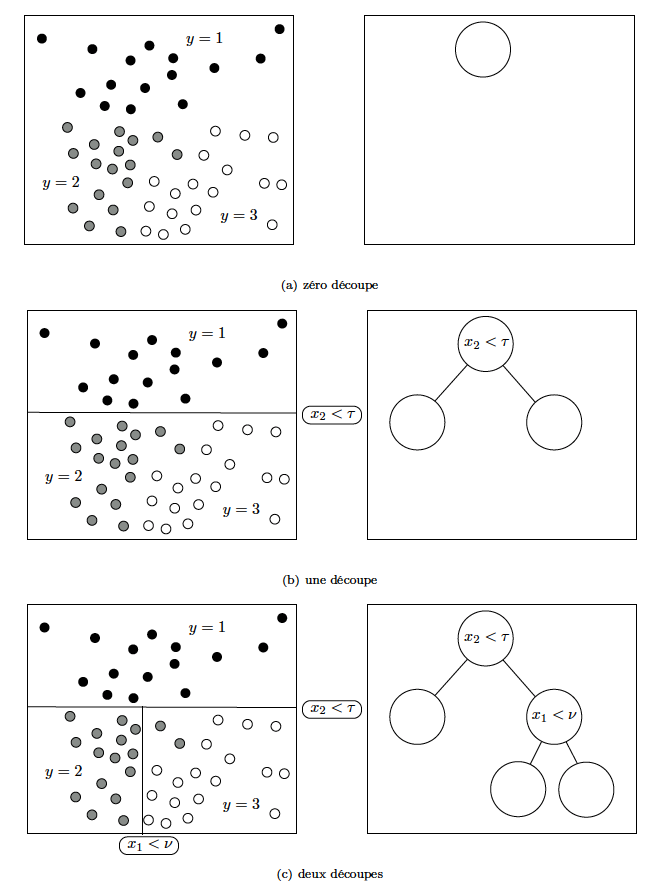
\includegraphics[width=8cm]{tree.png}

Il faut maintenant définir une règle pour décider où l’on doit faire la nouvelle découpe (splitting). 
Ce choix est crucial et n’est pas unique. 

Pour cela on utilise une fonction qui mesure “l’impureté”, que l’on
note $H$ associée à une partition. On cherche alors la découpe (variable/seuil) qui produit une partition la plus pure possible selon le critère $H$.\\

On cherche à réaliser la partition qui minimise l'impureté, en choisissant la dimension $j$, et le seuil $\tau$. Mathématiquement il s’agit de résoudre :

$$ \underset{j \in \llbracket 1; p \rrbracket, \tau \in \mathbb{R}}{arg min} \hat q_{j,\tau} H(G(j,\tau)) + (1-\hat q_{j,\tau})H(D(j,\tau))$$

où $ \hat q_{j,\tau} $ est la proportion des observations qui tombent dans $G(j,\tau)$: 
$$
\hat q_{j,\tau} = 
\frac{|\{ i \in  \llbracket 1; n \rrbracket : x_i \in G(j, \tau) \}|}
{|\{ i' \in  \llbracket 1; n \rrbracket : x_{i'} \in G(j, \tau) \cup D(j, \tau) \}|}
$$
et $H$ est la mesure d'impureté, en général $H$ est:
\begin{itemize}
\item l’indice de Gini:
$$ \sum_{k=1}^K \hat p_k (R) (1- \hat p_k(R)) $$
\item ou l'entropie:
$$ - \sum_{k=1}^K \hat p_k(R) log(\hat p_k(R)) $$
\end{itemize}
où pour tout ensemble $ R \subset \mathbb{R}^p$ et toute étiquette $k$ on note $\hat p_k(R)$ la proportion d’observations qui ont $k$ comme étiquette (numérotées de 1 à $K$), i.e.:
$$
\hat p_k(R) = 
\frac{ | \{ i \in \llbracket 1; n \rrbracket : x_i \in R, y_i = k  \} |  }
{| \{ i \in \llbracket 1; n \rrbracket : x_i \in R  \} | } 
$$

\subsubsection{Méthodes de choix de paramètres - Sélection de modèle}

Il est rare de disposer en pratique d’un ensemble de test (on préfère inclure le plus grand nombre de
données dans l’ensemble d’apprentissage), c’est au praticien de garder une partie de ces données à cet
effet. \\

Pour sélectionner un modèle ou un paramètre tout en considérant le plus grand nombre d’exemples
possibles pour l’apprentissage, on utilise généralement une sélection par validation croisée. 

\subsubsection{Reste à faire}

Expliquer le 'pruning'.\\

Expliquer comment on recherche l'optimum à chaque itération.\\

Expliquer avantages et inconvénients.\\

Expliquer le choix des critères pour éviter l'overfitting.

\subsubsection{Synthèse}

\subsubsection{Aller plus loin}

\url{http://scikit-learn.org/stable/modules/tree.html}






\pagebreak
\section{Méthodes ensemblistes}
\subsection{Vue d'ensemble}
Remark:
I Machine Learning not so "automatic": too many
hyperparameters to tune


2. meta-learning: a procedure to automatically use a base
classier/regressor even weak to produce a performant
classier/regressor


3. committee learning or wisdom of the crowd: better results
are obtained by combining the predictions of a set of diverse
classiers/regressors


4. ensemble learning: Improve upon a single predictor by
building an ensemble of predictors (with no hyperparameter)


\subsection{Ensemble learning: committee based methods}

Au lieu d'un seul classifieur, on combine les prédictions d'un ensemble de classifieurs différents pour un individu $x$. 
$$ C_1(x), C_2(x), ... , C_M(x)$$
(les classifieurs ont été préalablement entraînés sur l'ensemble d'apprentissage $\mathcal{D}_n$)\\


La classe que l'on prédit peut être, dans le cas de classe binaires avec $\mathcal{Y} = \{-1,1\}$:
\begin{itemize}
\item un vote à la majorité:
$$ C_{maj} = sign \left(  \sum_{m=1}^M C_m(x) \right) $$
\item un vote à la majorité avec poids:
$$ C_{maj} = sign \left(  \sum_{m=1}^M \alpha_m C_m(x) \right) $$
avec $\alpha_i > 0$ et, $ \sum_i \alpha_i = 1$
\end{itemize}

\subsection{Bagging}
Bootstrap aggregating technique.\\

Entraînement d'un unique classifieur $C$ sur une multitude d'échantillons obtenus par bootstrap.\\

Etant donné un ensemble d'apprentissage $\mathcal{D}_n$:

\begin{enumerate}
\item On génère $B \geq 1 $ échantillons $\mathcal{D}_n^{*(b)}$,
\item Pour $b \in \llbracket 1; B \rrbracket$, on entraîne le classifieur $C$ sur $\mathcal{D}_n^{*(b)}$, grâce à quoi nous obtenons le classifieur entraîné $C^{*(b)}$
\item On aggrège nos prédictions avec un vote à la majorité:
$$ C_{bag} = sign \left(  \sum_{b=1}^B C^{*(b)} \right) $$
\end{enumerate}

\subsubsection{Avantages}
Bagging can dramatically reduce the variance of unstable
procedures (ex: decision trees)

Variance reduction may lead to a smaller test error

Regression setup: $f_{bag}(x) = E[f^*(x)]$ (expectation taken over the training data)

In classication:
bagging a good classier makes it better, and ...
bagging a bad classier can make it worse!

\subsection{Boosting: AdaBoost = adaptive boosting}

Le principe est d'attribuer des poids aux individus de notre échantillon en fonction de leur erreur de prédiction: plus leur prédiction est fausse, plus on augmente leur poids.
Puis on aggrège à la fin les classifieurs obtenus lors des multiples itérations par une fonction non-linéaire.

\begin{enumerate}
\item initialisation avec des poids uniformes: 
\item pour m allant de 1 à M:
\begin{itemize}
\item entraînement du classifieur sur les individus en tenant compte du poids assigné
\end{itemize}
\end{enumerate}

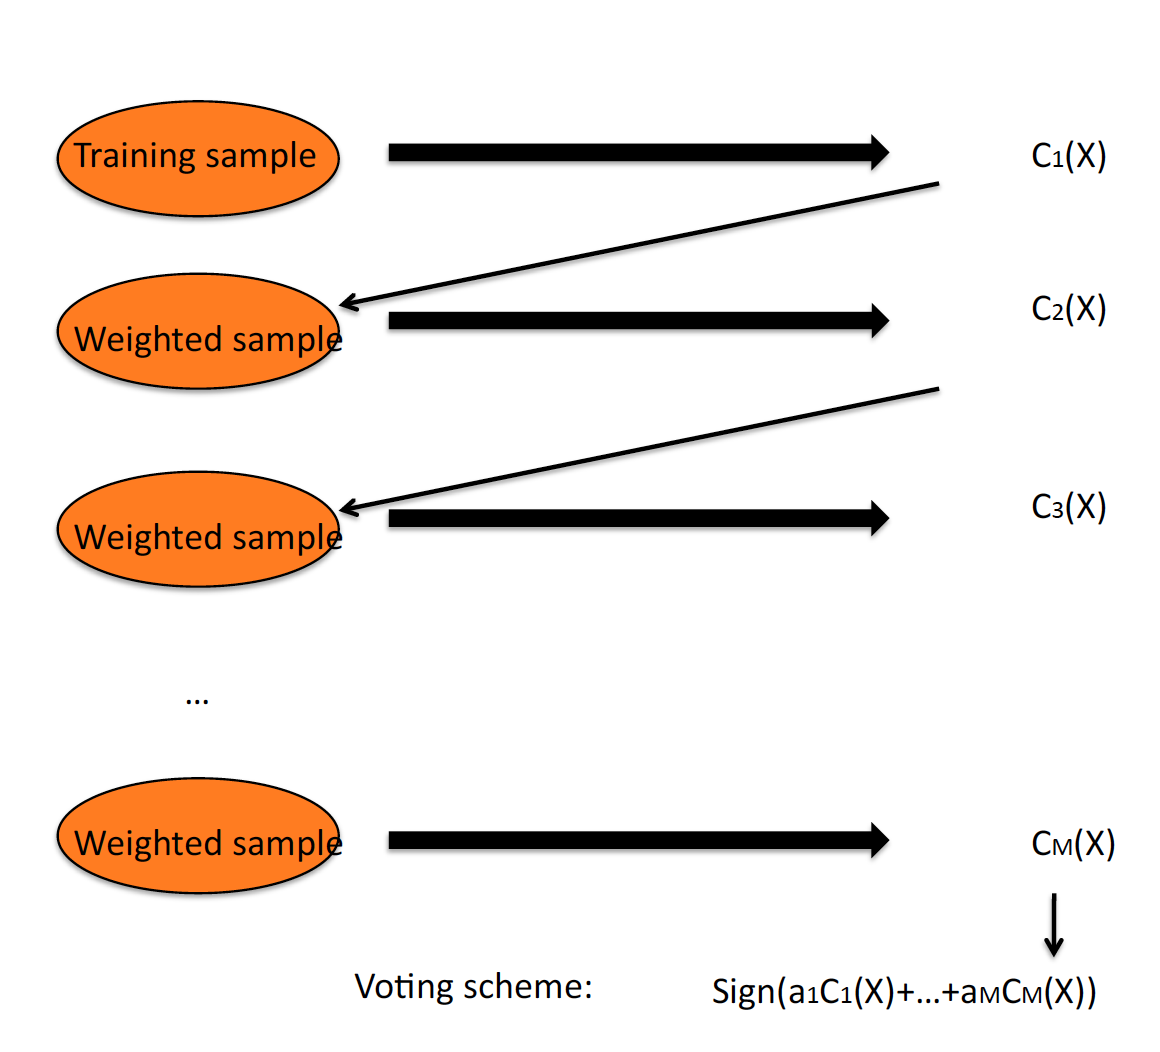
\includegraphics[width=13cm]{Adaboost.png}

\subsubsection{Avantages}


\subsection{Random forests}






\pagebreak
\section{Annexes classification}

\subsubsection{Preuves pour borner l'excès de risque d'un classifieur d'apres la complexité de la classe $\mathcal{F}$}

Quelques outils probabilistes.

\textbf{Inégalité de Markov}
The simplest inequality to bound the difference between a random variable and its expected value is Markov's inequality: for any nonnegative random variable $X$, and $t > 0$:
$$\mathbb{P}\{{X>t}\}\leq \frac{\mathbb{E}(X)}{t}$$

\textbf{Inégalité de Chebyshev:}

if $X$ is an arbitrary random variable and $t > 0$, then:

\textbf{Inégalité de Hoeffding}



\subsubsection{Méthodes de sélection de modèle par pénalisation}
\label{Detail_penalisation}


\textbf{Régulariser par la borne fournie par l'inégalité de VC}
A faire\\

\textbf{Le $C_P$ de Mallows pour la régression linéaire, et régression logistique}
Ce fut le premier critère visant une meilleure estimation de l'erreur de prédiction que la seule considération de l'erreur d'ajeustement (ou le $R^2$) dans le modèle linaire.
$$ C_P = \hat R_n(\hat f_n)+2 \frac{d}{n} \hat s^2$$
Où d est le nombre de paramères du modèle (dimension de $\mathcal{F}$), et $\hat s^2$ une estimation de la variance de l'erreur par un modèle de faible biais (on le fait avec un modèle simple, qui minimise le biais).\\
\url{http://citeseerx.ist.psu.edu/viewdoc/download?doi=10.1.1.544.4177&rep=rep1&type=pdf}
\textbf{A revoir car pas bien compris}\\

\textbf{Le critère d'Akaike (AIC), pour log-vraisemblance}
Il s'applique à tout modèle estimé par minimisation d'une log-vraisemblance.
$$ AIC = -2 log(\mathcal{L})+2\frac{d}{n}$$
Suppose que la famille de densités considérées pour modéliser la loi de Y, contient la "vraie" densité. Dans le cas gaussien à variance connue, moindres carrés et débiance coincident, AIC est équivalent à $C_P$.

Il est facile de choisir le modèle présentant le plus faible AIC parmi ceux considérés, ce qui revient à minimiser un critère de vraisemblance pénalisée.

Celui ci n'est vérifié qu'asymptotiquement d'où la motivation de proposer des critères modifiés plus adaptés à de petits échantillons.\\

\textbf{Bayesian information criterion}

\subsection{En cours d'écriture}


\subsection{TODO}

\begin{outline}
\1 Sélection de modèle: à refaire plus clairement
\1 Bayes, LDA, regression log lin, perceptron, synthèse de comparaison
\1 SVM à faire, et nuSVM/SVC
\1 Perceptron multicouche
\1 algorithmes de résolution de problèmes de m-estimation: ML, LS
\2 newton
\2 descente de gradient
\2 descente par coordonnées
\end{outline}
\bibliographystyle{alpha}
\bibliography{sample}
\end{document}